\documentclass[11pt,a4paper]{article}
\usepackage[margin=1in]{geometry}
\usepackage{graphicx}
\usepackage{booktabs}
\usepackage{amsmath}
\usepackage{hyperref}
\usepackage[numbers]{natbib}
\usepackage{listings}
\usepackage{xcolor}
\usepackage{float}
\usepackage{subcaption}
\usepackage{longtable}
\usepackage{multirow}

% Code listing style
\lstset{
    basicstyle=\ttfamily\small,
    keywordstyle=\color{blue},
    commentstyle=\color{gray},
    stringstyle=\color{orange},
    frame=single,
    breaklines=true,
    language=Python,
    showstringspaces=false,
    numbers=left,
    numberstyle=\tiny\color{gray}
}

\title{Technical Appendix:\\Regime-Aware Experience Replay for Deep Reinforcement Learning in Portfolio Optimization}
\author{Prince Alexander John \\ University of Birmingham \\ School of Computer Science}
\date{March 2026}

\begin{document}
\maketitle

\tableofcontents
\newpage

% =============================================================================
\appendix

\section{Experimental Configuration}
\label{app:config}

This appendix provides complete hyperparameter specifications for all algorithms tested in our experiments. All experiments were conducted on a system with an NVIDIA RTX 5090 Laptop GPU (23.9GB VRAM), using Python 3.12.10, PyTorch 2.10.0 with CUDA 12.8, and Stable Baselines3 for algorithm implementations.

\subsection{TD3 Hyperparameters}

Twin Delayed DDPG (TD3) is our primary algorithm, achieving the best overall performance across all replay strategies.

\begin{table}[H]
\centering
\caption{TD3 Hyperparameters}
\label{tab:td3-params}
\begin{tabular}{lll}
\toprule
\textbf{Parameter} & \textbf{Value} & \textbf{Description} \\
\midrule
\multicolumn{3}{l}{\textit{Learning}} \\
learning\_rate & $3 \times 10^{-4}$ & Adam optimizer learning rate \\
batch\_size & 256 & Mini-batch size for gradient updates \\
buffer\_size & 1,000,000 & Replay buffer capacity \\
gamma ($\gamma$) & 0.99 & Discount factor \\
tau ($\tau$) & 0.005 & Soft update coefficient \\
\midrule
\multicolumn{3}{l}{\textit{TD3-Specific}} \\
policy\_delay & 2 & Policy updates per critic update \\
target\_policy\_noise & 0.2 & Noise added to target actions \\
target\_noise\_clip & 0.5 & Clipping range for target noise \\
\midrule
\multicolumn{3}{l}{\textit{Training}} \\
train\_freq & 4 & Steps between gradient updates \\
gradient\_steps & 1 & Gradient steps per update \\
learning\_starts & 10,000 & Steps before training begins \\
total\_timesteps & 500,000 & Total training steps \\
\midrule
\multicolumn{3}{l}{\textit{Network Architecture}} \\
net\_arch & [256, 256] & Hidden layer sizes (actor \& critic) \\
activation\_fn & ReLU & Activation function \\
\midrule
\multicolumn{3}{l}{\textit{Exploration}} \\
action\_noise & Normal & Gaussian exploration noise \\
noise\_std & 0.1 & Standard deviation of action noise \\
\bottomrule
\end{tabular}
\end{table}

\subsection{SAC Hyperparameters}

Soft Actor-Critic uses entropy regularization to encourage exploration. Our experiments revealed that SAC is incompatible with regime-aware replay due to entropy bias.

\begin{table}[H]
\centering
\caption{SAC Hyperparameters}
\label{tab:sac-params}
\begin{tabular}{lll}
\toprule
\textbf{Parameter} & \textbf{Value} & \textbf{Description} \\
\midrule
\multicolumn{3}{l}{\textit{Learning}} \\
learning\_rate & $3 \times 10^{-4}$ & Adam optimizer learning rate \\
batch\_size & 256 & Mini-batch size \\
buffer\_size & 1,000,000 & Replay buffer capacity \\
gamma ($\gamma$) & 0.99 & Discount factor \\
tau ($\tau$) & 0.005 & Soft update coefficient \\
\midrule
\multicolumn{3}{l}{\textit{SAC-Specific}} \\
ent\_coef & auto & Automatic entropy tuning \\
target\_entropy & auto & Automatic target entropy \\
\midrule
\multicolumn{3}{l}{\textit{Training}} \\
train\_freq & 4 & Steps between gradient updates \\
gradient\_steps & 1 & Gradient steps per update \\
learning\_starts & 10,000 & Steps before training begins \\
total\_timesteps & 500,000 & Total training steps \\
\midrule
\multicolumn{3}{l}{\textit{Network Architecture}} \\
net\_arch & [256, 256] & Hidden layer sizes \\
\bottomrule
\end{tabular}
\end{table}

\subsection{PPO Hyperparameters}

Proximal Policy Optimization is an on-policy algorithm that does not use experience replay. We make it regime-aware by augmenting observations with regime information.

\begin{table}[H]
\centering
\caption{PPO Hyperparameters}
\label{tab:ppo-params}
\begin{tabular}{lll}
\toprule
\textbf{Parameter} & \textbf{Value} & \textbf{Description} \\
\midrule
\multicolumn{3}{l}{\textit{Learning}} \\
learning\_rate & $3 \times 10^{-4}$ & Adam optimizer learning rate \\
batch\_size & 64 & Mini-batch size \\
n\_steps & 2,048 & Steps to collect before update \\
n\_epochs & 10 & Epochs per update \\
gamma ($\gamma$) & 0.99 & Discount factor \\
\midrule
\multicolumn{3}{l}{\textit{PPO-Specific}} \\
gae\_lambda & 0.95 & GAE parameter \\
clip\_range & 0.2 & PPO clipping parameter \\
vf\_coef & 0.5 & Value function loss coefficient \\
ent\_coef & 0.01 & Entropy bonus coefficient \\
max\_grad\_norm & 0.5 & Gradient clipping threshold \\
\midrule
\multicolumn{3}{l}{\textit{Network Architecture}} \\
net\_arch & [256, 256] & Hidden layer sizes \\
\midrule
\multicolumn{3}{l}{\textit{Regime-Awareness}} \\
add\_regime\_to\_obs & True & Augment observations with regime \\
\bottomrule
\end{tabular}
\end{table}

\subsection{Rainbow DQN Hyperparameters}

Rainbow combines multiple DQN improvements. We use a custom implementation with distributional RL, prioritized replay, and dueling networks.

\begin{table}[H]
\centering
\caption{Rainbow DQN Hyperparameters}
\label{tab:rainbow-params}
\begin{tabular}{lll}
\toprule
\textbf{Parameter} & \textbf{Value} & \textbf{Description} \\
\midrule
\multicolumn{3}{l}{\textit{Learning}} \\
learning\_rate & $6.25 \times 10^{-5}$ & Adam optimizer learning rate \\
batch\_size & 32 & Mini-batch size \\
buffer\_size & 200,000 & Replay buffer capacity \\
gamma ($\gamma$) & 0.99 & Discount factor \\
\midrule
\multicolumn{3}{l}{\textit{Distributional RL}} \\
n\_atoms & 51 & Number of atoms in distribution \\
v\_min & -10.0 & Minimum value support \\
v\_max & 10.0 & Maximum value support \\
n\_steps & 3 & Multi-step returns \\
\midrule
\multicolumn{3}{l}{\textit{Prioritized Replay}} \\
per\_alpha & 0.6 & Priority exponent \\
per\_beta & 0.4 & Importance sampling exponent \\
\midrule
\multicolumn{3}{l}{\textit{Training}} \\
target\_update\_freq & 8,000 & Target network update frequency \\
learning\_starts & 20,000 & Steps before training begins \\
train\_freq & 4 & Steps between gradient updates \\
total\_timesteps & 500,000 & Total training steps \\
\midrule
\multicolumn{3}{l}{\textit{Network Architecture}} \\
hidden\_dims & [256, 256] & Hidden layer sizes \\
noisy\_sigma & 0.5 & NoisyNet initial $\sigma$ \\
\bottomrule
\end{tabular}
\end{table}

\subsection{Environment Configuration}

\begin{table}[H]
\centering
\caption{Trading Environment Configuration}
\label{tab:env-config}
\begin{tabular}{lll}
\toprule
\textbf{Parameter} & \textbf{Value} & \textbf{Description} \\
\midrule
\multicolumn{3}{l}{\textit{Assets}} \\
universe & SPY, QQQ, TLT, GLD, BIL & 5-asset portfolio \\
initial\_capital & \$1,000,000 & Starting portfolio value \\
\midrule
\multicolumn{3}{l}{\textit{Costs}} \\
transaction\_cost & 0.001 (10 bps) & Per-trade cost \\
\midrule
\multicolumn{3}{l}{\textit{Reward}} \\
reward\_scaling & 1.0 & Reward multiplier \\
$\lambda_{\text{cost}}$ & 1.0 & Transaction cost penalty coefficient \\
$\lambda_{\text{risk}}$ & 0.1 & Drawdown penalty coefficient \\
DD\_threshold & 0.10 & Drawdown threshold before penalty \\
\midrule
\multicolumn{3}{l}{\textit{Data Splits}} \\
train\_period & 2010-01-01 to 2019-12-31 & Training data \\
val\_period & 2020-01-01 to 2021-12-31 & Validation data \\
test\_period & 2022-01-01 to 2023-12-31 & Test data \\
\bottomrule
\end{tabular}
\end{table}


\section{Research Hypotheses}
\label{app:hypotheses}

Table~\ref{tab:hypotheses} summarises the six research hypotheses that guided our experimental programme. Each hypothesis is mapped to the experiment(s) designed to test it, along with the outcome based on our results.

\begin{table}[H]
\centering
\small
\caption{Research hypotheses, associated experiments, and outcomes.}
\label{tab:hypotheses}
\begin{tabular}{@{}cp{5.2cm}cp{6.2cm}@{}}
\toprule
\textbf{ID} & \textbf{Hypothesis} & \textbf{Test} & \textbf{Outcome} \\
\midrule
H1 & Regime-aware replay improves risk-adjusted returns vs standard uniform replay & E1 & \textbf{Not supported.} Standard replay yields the best Sharpe (+0.632); no regime-aware strategy significantly outperforms it ($p > 0.05$) \\[6pt]
H2 & Balanced sampling reduces performance variance across market regimes & E1, E2 & \textbf{Not supported.} Balanced sampling does not reduce cross-regime variance and actively harms SAC ($d = -2.95$) \\[6pt]
H3 & Inverse-frequency sampling improves bear market performance & E2 & \textbf{Not supported.} TD3's bear market advantage stems from the algorithm, not the sampling strategy \\[6pt]
H4 & Current-focused sampling improves short-term adaptability & E2 & \textbf{Partially supported.} TD3 current-focused achieves the highest bear regime Sharpe (+1.07) but ranks second overall \\[6pt]
H5 & Benefits are consistent across all four algorithms & E1 & \textbf{Rejected.} SAC is fundamentally incompatible with non-uniform replay; effects are algorithm-dependent \\[6pt]
H6 & Robust to moderate noise ($\leq$20\%) in regime detection & E3 & \textbf{Supported.} No significant degradation up to 30\% noise ($p > 0.05$) \\
\bottomrule
\end{tabular}
\end{table}


\section{Full Results Tables}
\label{app:results}

This appendix provides complete result tables for all seven experiments. The primary metric is the annualized Sharpe ratio computed on the 2022--2023 test period. Secondary metrics include the Sortino ratio (return per unit of downside risk), Calmar ratio (annualized return divided by maximum drawdown), and cumulative return. MDD denotes maximum drawdown. Val--Test Gap is the difference between validation and test Sharpe ratios; larger gaps indicate greater overfitting.

\subsection{E1: Replay Strategy Comparison (100 Runs)}

\begin{table}[H]
\centering
\caption{Complete E1 results: 4 algorithms $\times$ 5 strategies $\times$ 5 seeds. Sorted by algorithm, then strategy.}
\label{tab:e1-full}
\resizebox{\textwidth}{!}{%
\begin{tabular}{@{}llcccccccc@{}}
\toprule
\textbf{Algorithm} & \textbf{Strategy} & \textbf{Sharpe} & \textbf{$\pm$ Std} & \textbf{Sortino} & \textbf{Ret. (\%)} & \textbf{Calmar} & \textbf{Val Sharpe} & \textbf{MDD (\%)} & \textbf{Gap} \\
\midrule
PPO & adaptive & +0.281 & 0.185 & +0.442 & +8.1 & +0.226 & 1.359 & 19.4 & 1.078 \\
PPO & balanced & +0.168 & 0.205 & +0.261 & +5.1 & +0.133 & 1.503 & 21.1 & 1.335 \\
PPO & current\_focused & +0.325 & 0.293 & +0.509 & +8.3 & +0.314 & 1.411 & 16.9 & 1.086 \\
PPO & inverse\_freq & +0.212 & 0.236 & +0.330 & +5.8 & +0.159 & 1.876 & 20.8 & 1.664 \\
PPO & standard & +0.289 & 0.288 & +0.455 & +7.6 & +0.245 & 1.313 & 17.6 & 1.024 \\
\midrule
Rainbow & adaptive & $-$0.007 & 0.057 & $-$0.010 & $-$0.2 & $-$0.003 & 1.321 & 20.5 & 1.328 \\
Rainbow & balanced & +0.060 & 0.046 & +0.093 & +1.3 & +0.035 & 1.345 & 19.1 & 1.285 \\
Rainbow & current\_focused & $-$0.024 & 0.073 & $-$0.037 & $-$0.5 & $-$0.014 & 1.408 & 20.7 & 1.432 \\
Rainbow & inverse\_freq & +0.091 & 0.126 & +0.145 & +2.2 & +0.059 & 1.349 & 20.0 & 1.258 \\
Rainbow & standard & +0.062 & 0.080 & +0.098 & +1.5 & +0.039 & 1.462 & 20.1 & 1.400 \\
\midrule
SAC & adaptive & +0.171 & 0.213 & +0.268 & +4.1 & +0.113 & 1.165 & 18.6 & 0.994 \\
SAC & balanced & $-$0.014 & 0.173 & $-$0.012 & $-$0.3 & $-$0.006 & 1.337 & 21.7 & 1.351 \\
SAC & current\_focused & +0.084 & 0.205 & +0.127 & +2.0 & +0.057 & 1.213 & 20.9 & 1.129 \\
SAC & inverse\_freq & +0.134 & 0.164 & +0.205 & +3.3 & +0.091 & 1.341 & 19.1 & 1.207 \\
SAC & standard & +0.458 & 0.146 & +0.728 & +13.3 & +0.374 & 1.702 & 17.1 & 1.244 \\
\midrule
TD3 & adaptive & +0.501 & 0.127 & +0.795 & +16.1 & +0.496 & 1.444 & 16.3 & 0.943 \\
TD3 & balanced & +0.438 & 0.162 & +0.661 & +14.4 & +0.393 & 1.415 & 18.6 & 0.977 \\
TD3 & current\_focused & +0.620 & 0.333 & +0.999 & +19.8 & +0.654 & 1.725 & 17.3 & 1.105 \\
TD3 & inverse\_freq & +0.254 & 0.188 & +0.403 & +7.9 & +0.210 & 1.608 & 20.0 & 1.354 \\
TD3 & standard & \textbf{+0.632} & 0.166 & +0.998 & +19.7 & +0.645 & 1.537 & 15.2 & \textbf{0.905} \\
\bottomrule
\end{tabular}%
}
\end{table}

\subsection{E3: Robustness to Noisy Regime Detection (36 Runs)}

TD3 only, with regime label noise at 0\%, 10\%, 20\%, and 30\%.

\begin{table}[H]
\centering
\caption{E3 results: TD3 with varying regime detection noise levels (3 seeds per config).}
\label{tab:e3-full}
\resizebox{\textwidth}{!}{%
\begin{tabular}{@{}clccccccc@{}}
\toprule
\textbf{Noise} & \textbf{Strategy} & \textbf{Sharpe} & \textbf{$\pm$ Std} & \textbf{Sortino} & \textbf{Ret. (\%)} & \textbf{Val Sharpe} & \textbf{Gap} \\
\midrule
0\% & standard & +0.540 & 0.123 & +0.844 & +18.6 & 1.850 & 1.310 \\
0\% & balanced & +0.193 & 0.007 & +0.295 & +6.4 & 2.061 & 1.868 \\
0\% & inverse\_freq & +0.485 & 0.368 & +0.787 & +15.2 & 1.315 & 0.830 \\
\midrule
10\% & standard & +0.620 & 0.111 & +0.969 & +21.2 & 1.529 & 0.909 \\
10\% & balanced & +0.734 & 0.098 & +1.176 & +23.8 & 1.625 & 0.891 \\
10\% & inverse\_freq & +0.288 & 0.223 & +0.454 & +8.7 & 2.025 & 1.737 \\
\midrule
20\% & standard & +0.640 & 0.074 & +1.023 & +20.8 & 1.417 & 0.777 \\
20\% & balanced & +0.585 & 0.226 & +0.909 & +19.3 & 1.344 & 0.759 \\
20\% & inverse\_freq & +0.403 & 0.213 & +0.649 & +13.1 & 1.445 & 1.042 \\
\midrule
30\% & standard & +0.652 & 0.085 & +1.076 & +20.7 & 1.752 & 1.100 \\
30\% & balanced & +0.312 & 0.260 & +0.489 & +10.5 & 1.448 & 1.136 \\
30\% & inverse\_freq & +0.547 & 0.493 & +0.902 & +18.3 & 1.770 & 1.223 \\
\bottomrule
\end{tabular}%
}
\end{table}

\subsection{E4: Feature Ablation and E5: Detection Method}

\begin{table}[H]
\centering
\caption{E4 feature ablation (20 runs: PPO and SAC, 5 seeds each) and E5 detection method comparison (12 runs: SAC, 3 seeds each).}
\label{tab:e4e5}
\resizebox{\textwidth}{!}{%
\begin{tabular}{@{}lllccccccc@{}}
\toprule
\textbf{Exp} & \textbf{Config 1} & \textbf{Config 2} & \textbf{Sharpe} & \textbf{$\pm$ Std} & \textbf{Sortino} & \textbf{Ret. (\%)} & \textbf{MDD (\%)} & \textbf{Gap} \\
\midrule
\multicolumn{9}{l}{\textit{E4: Feature Ablation}} \\
E4 & PPO & full & +0.155 & 0.187 & +0.245 & +4.2 & 21.2 & 1.335 \\
E4 & PPO & reduced & +0.179 & 0.106 & +0.269 & +5.6 & 23.1 & 1.001 \\
E4 & SAC & full & $-$0.052 & 0.322 & $-$0.074 & $-$1.2 & 23.2 & 1.278 \\
E4 & SAC & reduced & +0.074 & 0.162 & +0.121 & +1.9 & 19.1 & 1.242 \\
\midrule
\multicolumn{9}{l}{\textit{E5: Detection Method (SAC only)}} \\
E5 & HMM & standard & +0.644 & 0.132 & +1.058 & +19.3 & 14.8 & 0.986 \\
E5 & HMM & balanced & $-$0.036 & 0.189 & $-$0.054 & $-$0.7 & 19.8 & 1.396 \\
E5 & Rule-based & standard & +0.617 & 0.087 & +0.995 & +18.3 & 13.7 & 1.164 \\
E5 & Rule-based & balanced & +0.001 & 0.079 & +0.005 & +0.0 & 21.8 & 1.234 \\
\bottomrule
\end{tabular}%
}
\end{table}

\subsection{E6: Sample Efficiency and E7: Timestep Ablation}

\begin{table}[H]
\centering
\caption{E6 sample efficiency (30 runs: TD3 and SAC at 1M timesteps, 5 seeds) and E7 timestep ablation (30 runs: TD3 only, 3 seeds).}
\label{tab:e6e7}
\resizebox{\textwidth}{!}{%
\begin{tabular}{@{}llcccccccc@{}}
\toprule
\textbf{Exp} & \textbf{Config} & \textbf{Strategy} & \textbf{Sharpe} & \textbf{$\pm$ Std} & \textbf{Sortino} & \textbf{Ret. (\%)} & \textbf{Val Sharpe} & \textbf{Gap} \\
\midrule
\multicolumn{9}{l}{\textit{E6: Sample Efficiency (1M timesteps)}} \\
E6 & TD3 & inverse\_freq & \textbf{+0.695} & 0.315 & +1.136 & +22.3 & 1.658 & 0.963 \\
E6 & TD3 & balanced & +0.567 & 0.222 & +0.913 & +18.6 & 1.764 & 1.197 \\
E6 & TD3 & standard & +0.432 & 0.425 & +0.686 & +13.8 & 1.525 & 1.093 \\
E6 & SAC & balanced & +0.338 & 0.291 & +0.549 & +9.1 & 1.255 & 0.917 \\
E6 & SAC & standard & +0.335 & 0.102 & +0.543 & +10.0 & 1.524 & 1.189 \\
E6 & SAC & inverse\_freq & +0.256 & 0.361 & +0.415 & +6.9 & 1.298 & 1.042 \\
\midrule
\multicolumn{9}{l}{\textit{E7: Timestep Ablation (TD3 only)}} \\
E7 & 100k & adaptive & +0.624 & 0.160 & +0.974 & +19.3 & 1.613 & 0.990 \\
E7 & 100k & standard & +0.550 & 0.194 & +0.886 & +17.1 & 1.655 & 1.105 \\
E7 & 200k & adaptive & +0.681 & 0.054 & +1.065 & +22.3 & 1.361 & 0.680 \\
E7 & 200k & standard & +0.373 & 0.312 & +0.593 & +11.8 & 1.193 & 0.820 \\
E7 & 300k & adaptive & +0.382 & 0.289 & +0.607 & +11.7 & 1.499 & 1.117 \\
E7 & 300k & standard & +0.356 & 0.122 & +0.576 & +11.4 & 1.457 & 1.101 \\
E7 & 400k & adaptive & +0.365 & 0.138 & +0.557 & +11.8 & 1.680 & 1.315 \\
E7 & 400k & standard & \textbf{+0.815} & 0.151 & +1.312 & +25.7 & 1.422 & \textbf{0.607} \\
E7 & 500k & adaptive & +0.738 & 0.195 & +1.152 & +24.6 & 1.586 & 0.848 \\
E7 & 500k & standard & +0.649 & 0.175 & +0.989 & +21.3 & 1.528 & 0.879 \\
\bottomrule
\end{tabular}%
}
\end{table}


\section{Statistical Analysis Details}
\label{app:stats}

This appendix provides the complete statistical analysis supporting the results in Section~\ref{sec:results}.

\textbf{Methodology.} All comparisons use Welch's $t$-test (unequal variances assumed) with each random seed treated as an independent observation ($n = 5$ per group for E1). We apply Bonferroni correction for multiple comparisons: with 16 pairwise tests in E1 (4 algorithms $\times$ 4 non-standard strategies vs standard), the corrected significance threshold is $\alpha = 0.05 / 16 = 0.003125$. Effect sizes are reported as Cohen's $d$, interpreted as: negligible ($< 0.2$), small ($0.2$--$0.5$), medium ($0.5$--$0.8$), and large ($> 0.8$).

\subsection{E1 Pairwise $t$-Tests: Strategy vs Standard}

\begin{table}[H]
\centering
\small
\caption{Pairwise $t$-tests comparing each regime-aware strategy against standard (uniform) replay within each algorithm. Bonferroni-corrected $\alpha = 0.003125$.}
\label{tab:e1-ttests}
\begin{tabular}{@{}llrrrl@{}}
\toprule
\textbf{Algorithm} & \textbf{Strategy} & \textbf{$t$-stat} & \textbf{$p$-value} & \textbf{Cohen's $d$} & \textbf{Bonf.} \\
\midrule
PPO & balanced & $-$0.76 & 0.469 & $-$0.48 & No \\
PPO & current\_focused & +0.20 & 0.849 & +0.12 & No \\
PPO & inverse\_freq & $-$0.46 & 0.659 & $-$0.29 & No \\
PPO & adaptive & $-$0.05 & 0.965 & $-$0.03 & No \\
\midrule
Rainbow & balanced & $-$0.06 & 0.954 & $-$0.04 & No \\
Rainbow & current\_focused & $-$1.78 & 0.112 & $-$1.13 & No \\
Rainbow & inverse\_freq & +0.42 & 0.685 & +0.27 & No \\
Rainbow & adaptive & $-$1.58 & 0.157 & $-$1.00 & No \\
\midrule
SAC & balanced & $-$4.66 & \textbf{0.00175} & $-$2.95 & \textbf{Yes} \\
SAC & current\_focused & $-$3.32 & 0.012 & $-$2.10 & No \\
SAC & inverse\_freq & $-$3.30 & 0.011 & $-$2.09 & No \\
SAC & adaptive & $-$2.49 & 0.041 & $-$1.57 & No \\
\midrule
TD3 & balanced & $-$1.86 & 0.099 & $-$1.18 & No \\
TD3 & current\_focused & $-$0.07 & 0.948 & $-$0.04 & No \\
TD3 & inverse\_freq & $-$3.37 & 0.010 & $-$2.13 & No \\
TD3 & adaptive & $-$1.40 & 0.203 & $-$0.88 & No \\
\bottomrule
\end{tabular}
\end{table}

All values are from pairwise Welch's $t$-tests on per-seed test Sharpe ratios ($n = 5$ per group). SAC balanced is the only Bonferroni-significant comparison ($p = 0.00175$, $d = -2.95$). SAC current-focused, inverse-frequency, and adaptive all show raw-significant declines ($p = 0.012$, $0.011$, and $0.041$ respectively, $|d| > 1.5$) that do not survive Bonferroni correction. Critically, all four SAC non-standard strategies show large negative effect sizes ($|d| > 1.0$), indicating a consistent pattern of degradation rather than random variation. No significant effects are observed for PPO after correction. TD3 inverse-frequency shows a raw-significant decline ($p = 0.010$, $d = -2.13$) that does not survive Bonferroni correction. TD3 adaptive also shows a large negative effect ($d = -0.88$, $p = 0.203$), consistent with its lower post-correction mean (+0.501 vs standard +0.632).

\subsection{E2 Bear Market Statistical Tests}

\begin{table}[H]
\centering
\small
\caption{Statistical tests for regime-level performance claims (E2).}
\label{tab:e2-stats}
\begin{tabular}{@{}lrrrl@{}}
\toprule
\textbf{Comparison} & \textbf{$p$-value} & \textbf{Cohen's $d$} & \textbf{Diff} & \textbf{Sig.} \\
\midrule
TD3 vs PPO (bear) & $2.4 \times 10^{-5}$ & +1.33 & +0.433 & Yes \\
TD3 vs SAC (bear) & $4.1 \times 10^{-7}$ & +1.66 & +0.586 & Yes \\
TD3 vs Rainbow (bear) & $7.6 \times 10^{-11}$ & +2.93 & +0.758 & Yes \\
SAC std vs bal (bear) & 0.032 & +1.68 & +0.551 & No \\
SAC std vs bal (bull) & 0.680 & +0.27 & +0.136 & No \\
SAC std vs bal (sideways) & 0.011 & +2.12 & +0.928 & No \\
TD3 adaptive vs std (bear) & 0.930 & $-$0.06 & $-$0.020 & No \\
\bottomrule
\end{tabular}
\end{table}

TD3's bear market superiority over all other algorithms is highly significant ($p < 0.001$ for all three comparisons), with large to very large effect sizes. SAC standard vs balanced shows large effects in bear and sideways regimes but does not reach significance after correction due to smaller sample sizes within each regime.

\subsection{Win Rate Analysis}

Win rates measure the proportion of seeds where a regime-aware strategy outperforms standard replay for the same algorithm (threshold: Sharpe difference $> 0.01$).

\begin{table}[H]
\centering
\small
\caption{Win rates: regime-aware strategy vs standard replay, by seed (5 seeds per comparison). A ``win'' requires a Sharpe difference $> 0.01$; differences $\leq 0.01$ are ties.}
\label{tab:win-rates}
\begin{tabular}{@{}llcccc@{}}
\toprule
\textbf{Algorithm} & \textbf{Strategy} & \textbf{Wins} & \textbf{Losses} & \textbf{Ties} & \textbf{Win Rate} \\
\midrule
PPO & balanced & 2 & 3 & 0 & 40\% \\
PPO & current\_focused & 2 & 3 & 0 & 40\% \\
PPO & inverse\_frequency & 1 & 4 & 0 & 20\% \\
PPO & adaptive & 1 & 4 & 0 & 20\% \\
\midrule
Rainbow & balanced & 2 & 3 & 0 & 40\% \\
Rainbow & current\_focused & 0 & 5 & 0 & 0\% \\
Rainbow & inverse\_frequency & 3 & 2 & 0 & 60\% \\
Rainbow & adaptive & 1 & 3 & 1 & 20\% \\
\midrule
SAC & balanced & 0 & 5 & 0 & 0\% \\
SAC & current\_focused & 0 & 5 & 0 & 0\% \\
SAC & inverse\_frequency & 0 & 5 & 0 & 0\% \\
SAC & adaptive & 0 & 5 & 0 & 0\% \\
\midrule
TD3 & balanced & 2 & 3 & 0 & 40\% \\
TD3 & current\_focused & 3 & 2 & 0 & 60\% \\
TD3 & inverse\_frequency & 0 & 5 & 0 & 0\% \\
TD3 & adaptive & 1 & 4 & 0 & 20\% \\
\bottomrule
\end{tabular}
\end{table}

SAC's 0\% win rate across all four non-standard strategies (losing on all 5 seeds in each case) provides additional evidence for the incompatibility finding. TD3 adaptive achieves a 20\% win rate (1 of 5 seeds), consistent with its lower mean Sharpe (+0.501) compared to standard (+0.632) after the EMA decay bug fix. TD3 inverse-frequency shows a 0\% win rate, mirroring its near-significant decline in Table~\ref{tab:e1-ttests}.


\section{All Figures}
\label{app:figures}

This appendix collects all experimental figures. Figures referenced in the main report are reproduced here for completeness alongside additional visualizations.

\subsection{E1: Replay Strategy Comparison}

\begin{figure}[H]
    \centering
    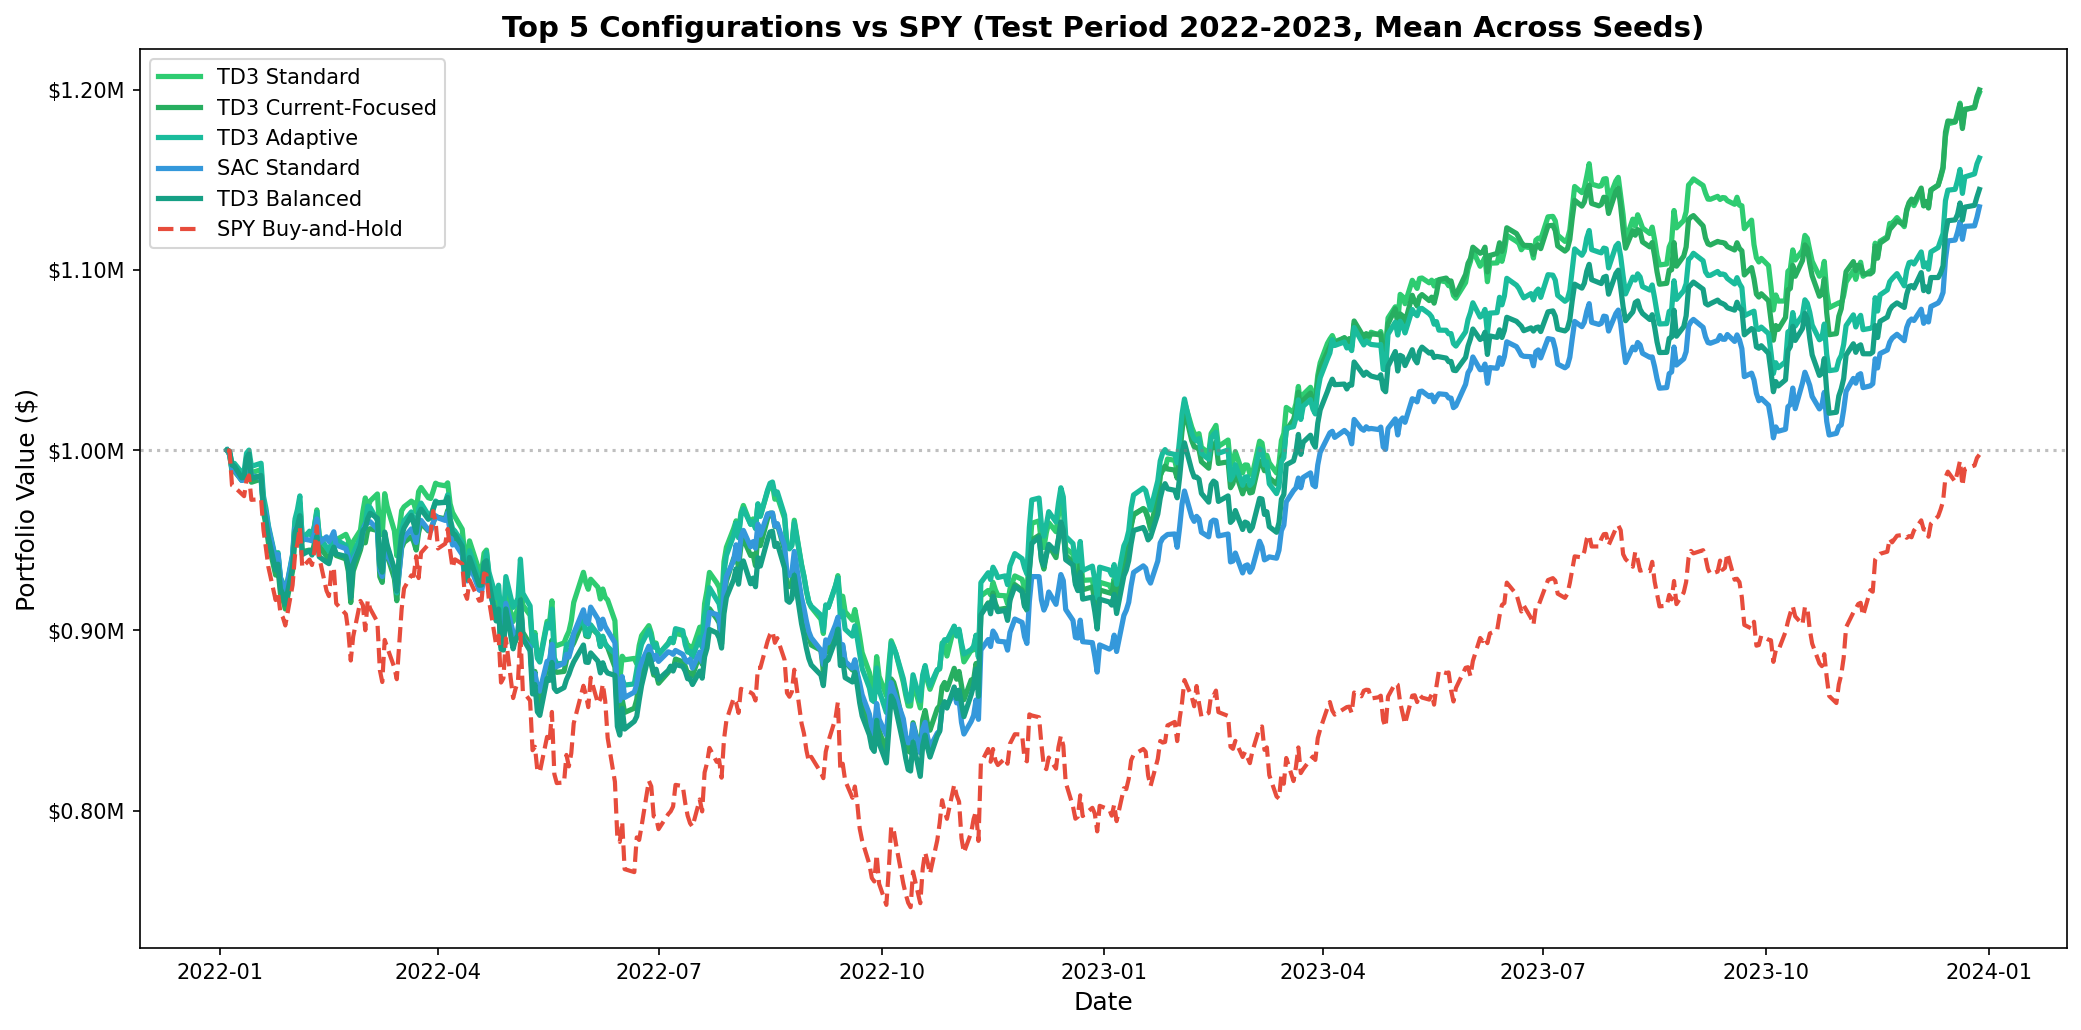
\includegraphics[width=0.88\textwidth]{figures/equity_curves_top5.png}
    \caption{Equity curves for the top 5 algorithm--strategy configurations versus the SPY benchmark on the 2022--2023 test period (mean across 5 seeds). Starting from \$1M, all five configurations outperform SPY. TD3 standard achieves the best Sharpe ratio of +0.632 with a maximum drawdown of 15.2\% compared to SPY's 25.3\%.}
    \label{fig:app-equity-td3}
\end{figure}

\begin{figure}[H]
    \centering
    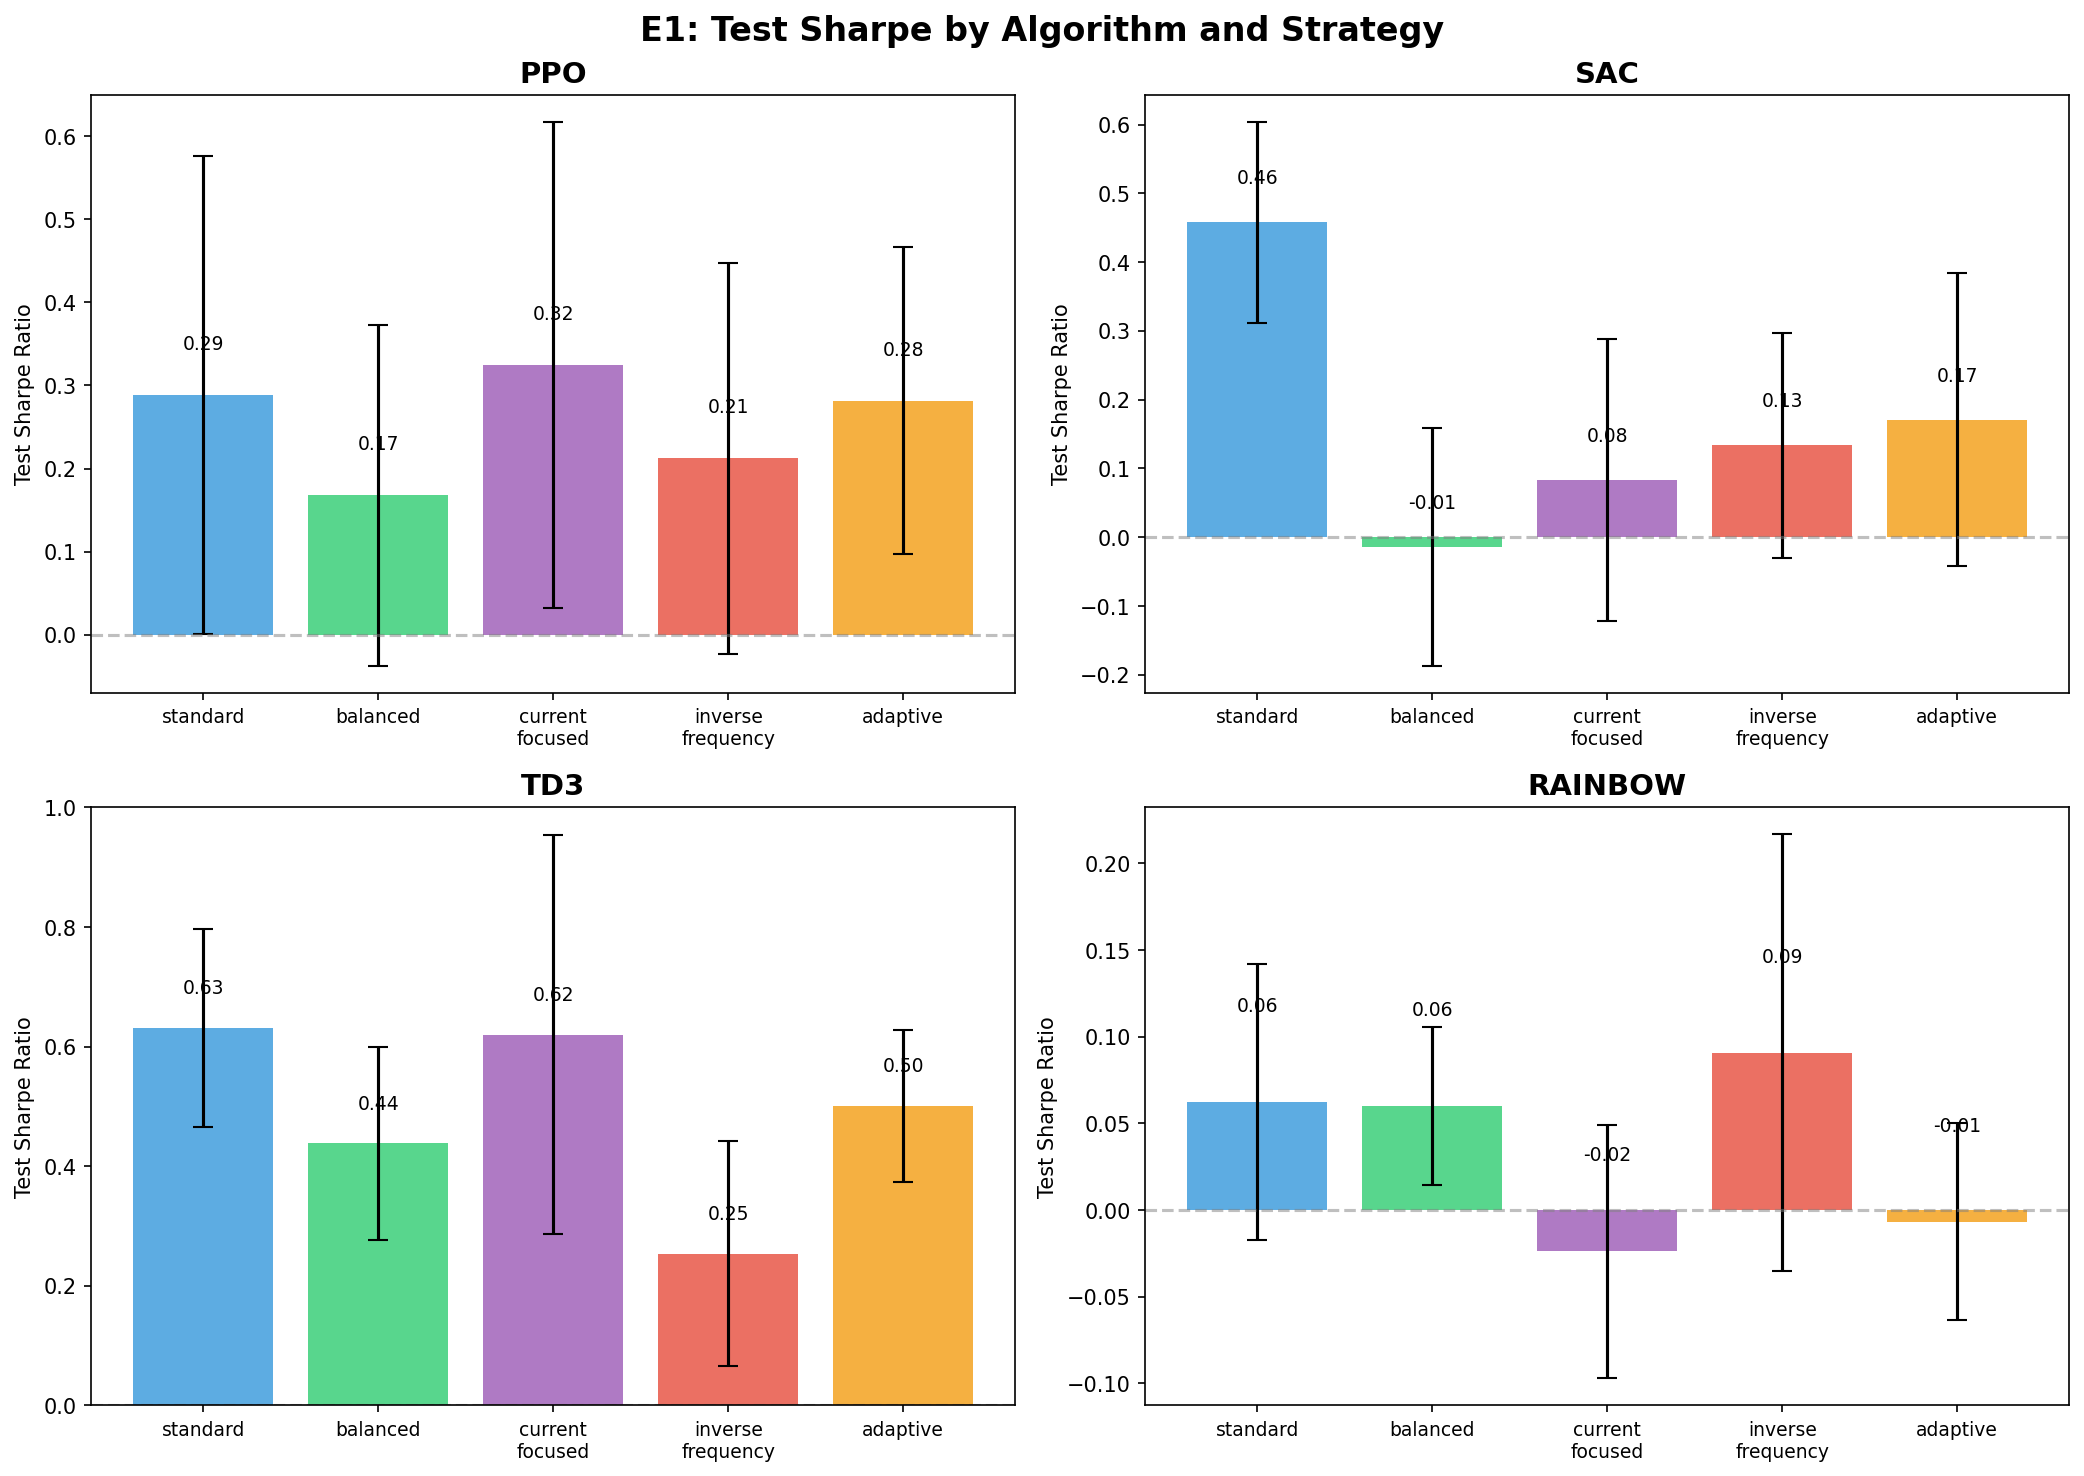
\includegraphics[width=0.88\textwidth]{figures/sharpe_by_strategy_bars.png}
    \caption{Test Sharpe ratios across all 20 algorithm--strategy combinations (E1, 5 seeds per bar, error bars show $\pm$1 standard deviation). TD3 performs consistently well across all strategies. SAC collapses with any non-standard replay. Rainbow DQN shows uniformly low test performance despite high validation Sharpe ratios, indicating severe overfitting.}
    \label{fig:app-sharpe-bars}
\end{figure}

\begin{figure}[H]
    \centering
    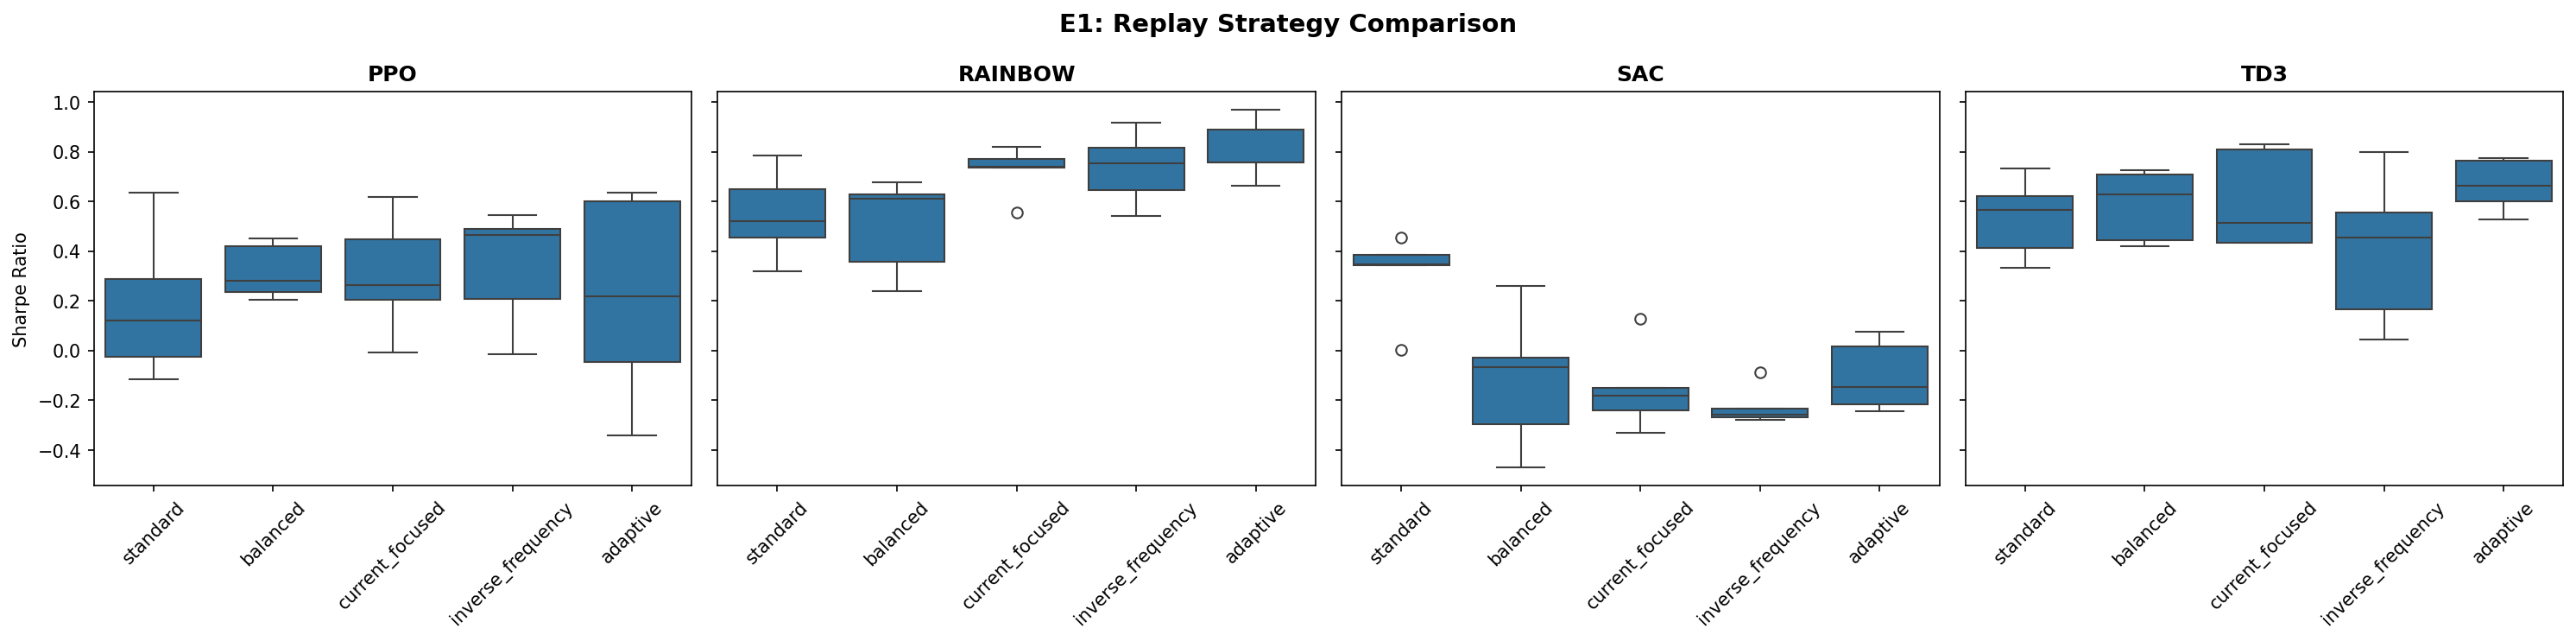
\includegraphics[width=0.88\textwidth]{figures/e1_sharpe_boxplots.png}
    \caption{Box plots of test Sharpe ratios by algorithm (E1, all strategies pooled). TD3 has the highest median and smallest interquartile range. SAC shows a bimodal distribution driven by the standard-vs-regime-aware split. Rainbow DQN clusters near zero with minimal variance.}
    \label{fig:app-boxplots}
\end{figure}

\begin{figure}[H]
    \centering
    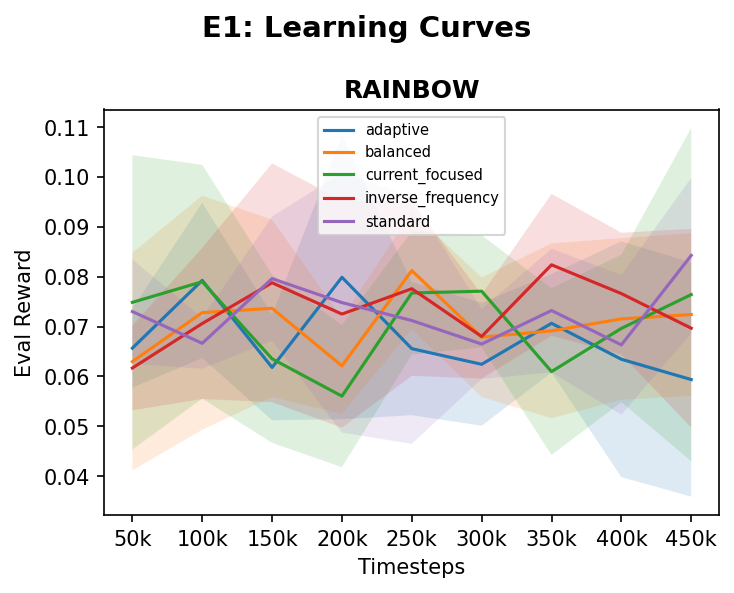
\includegraphics[width=0.88\textwidth]{figures/e1_learning_curves.png}
    \caption{Training learning curves for each algorithm (E1, averaged across strategies and seeds). TD3 and SAC converge within 300k timesteps, while PPO shows more gradual improvement. Rainbow DQN converges quickly on the training set but this does not translate to test performance.}
    \label{fig:app-learning}
\end{figure}

\subsection{E2: Regime-Level Analysis}

\begin{figure}[H]
    \centering
    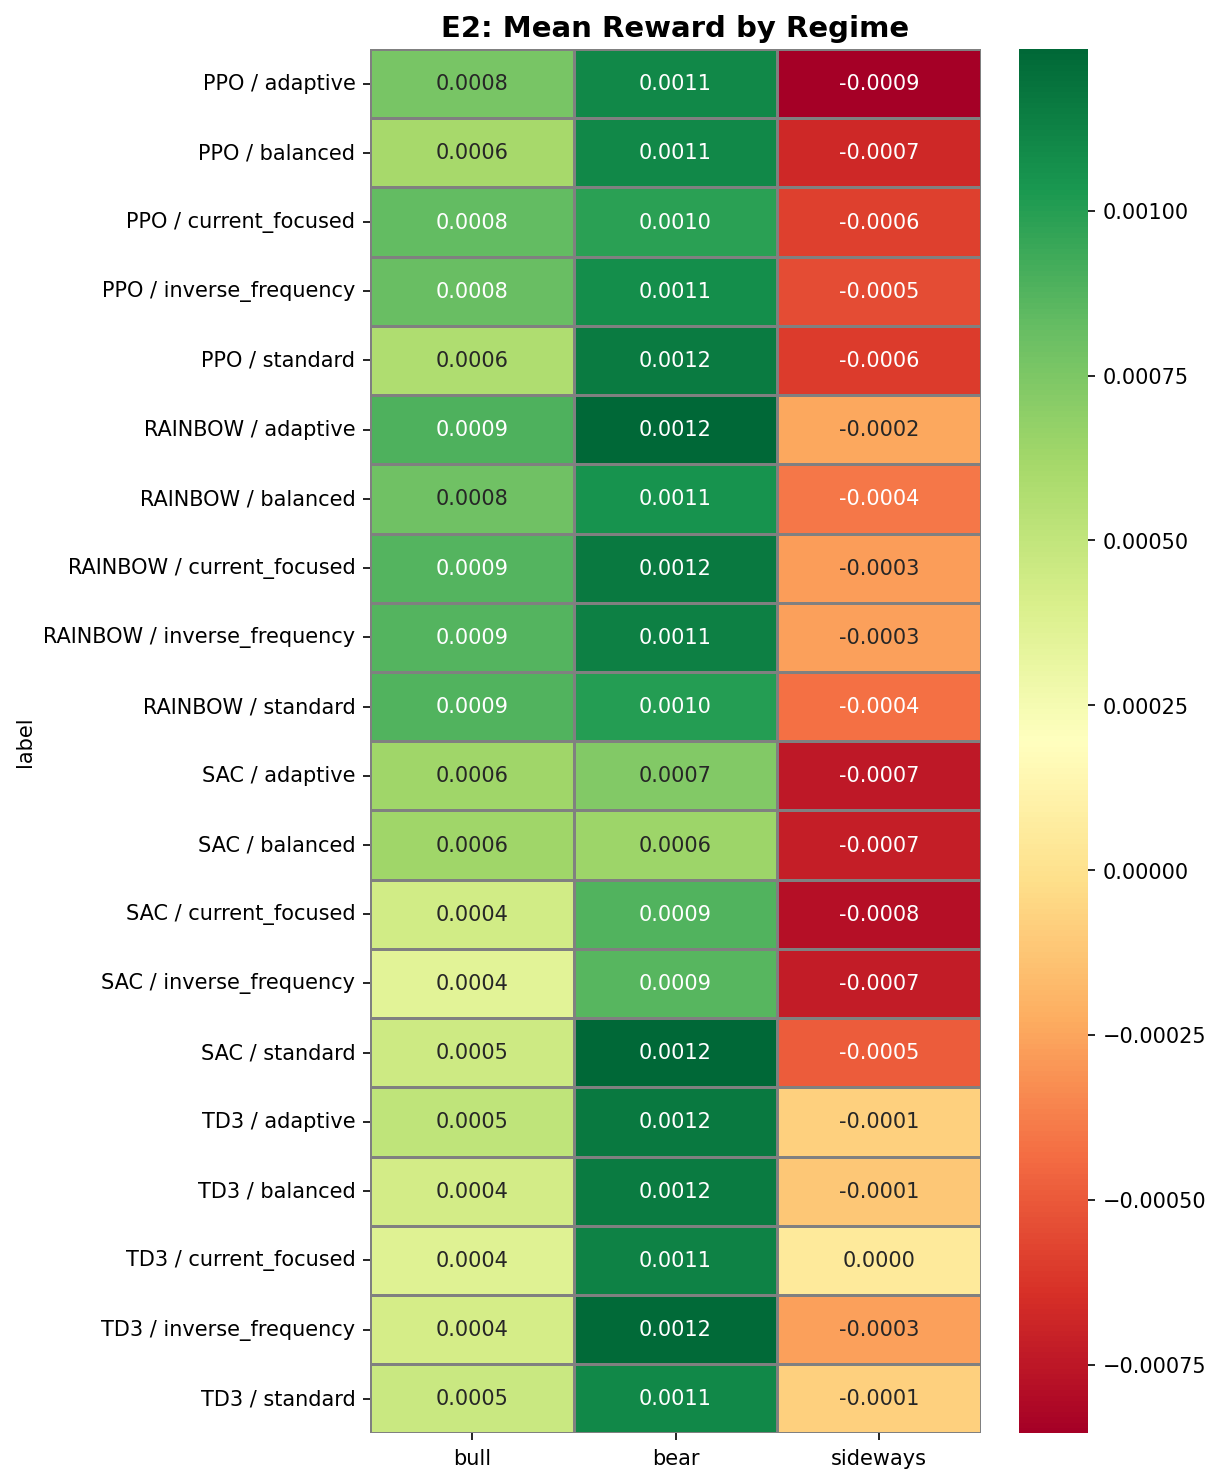
\includegraphics[width=0.88\textwidth]{figures/e2_regime_heatmap.png}
    \caption{Mean Sharpe ratio by algorithm and market regime (E2, aggregated across all strategies and seeds). TD3 dominates bear markets (+0.931 mean) while all algorithms profit in bull markets (+1.564 aggregate) and struggle in sideways conditions ($-1.286$ aggregate). The colour intensity reveals TD3's unique ability to extract positive returns from bear-market dynamics.}
    \label{fig:app-regime-heatmap}
\end{figure}

\begin{figure}[H]
    \centering
    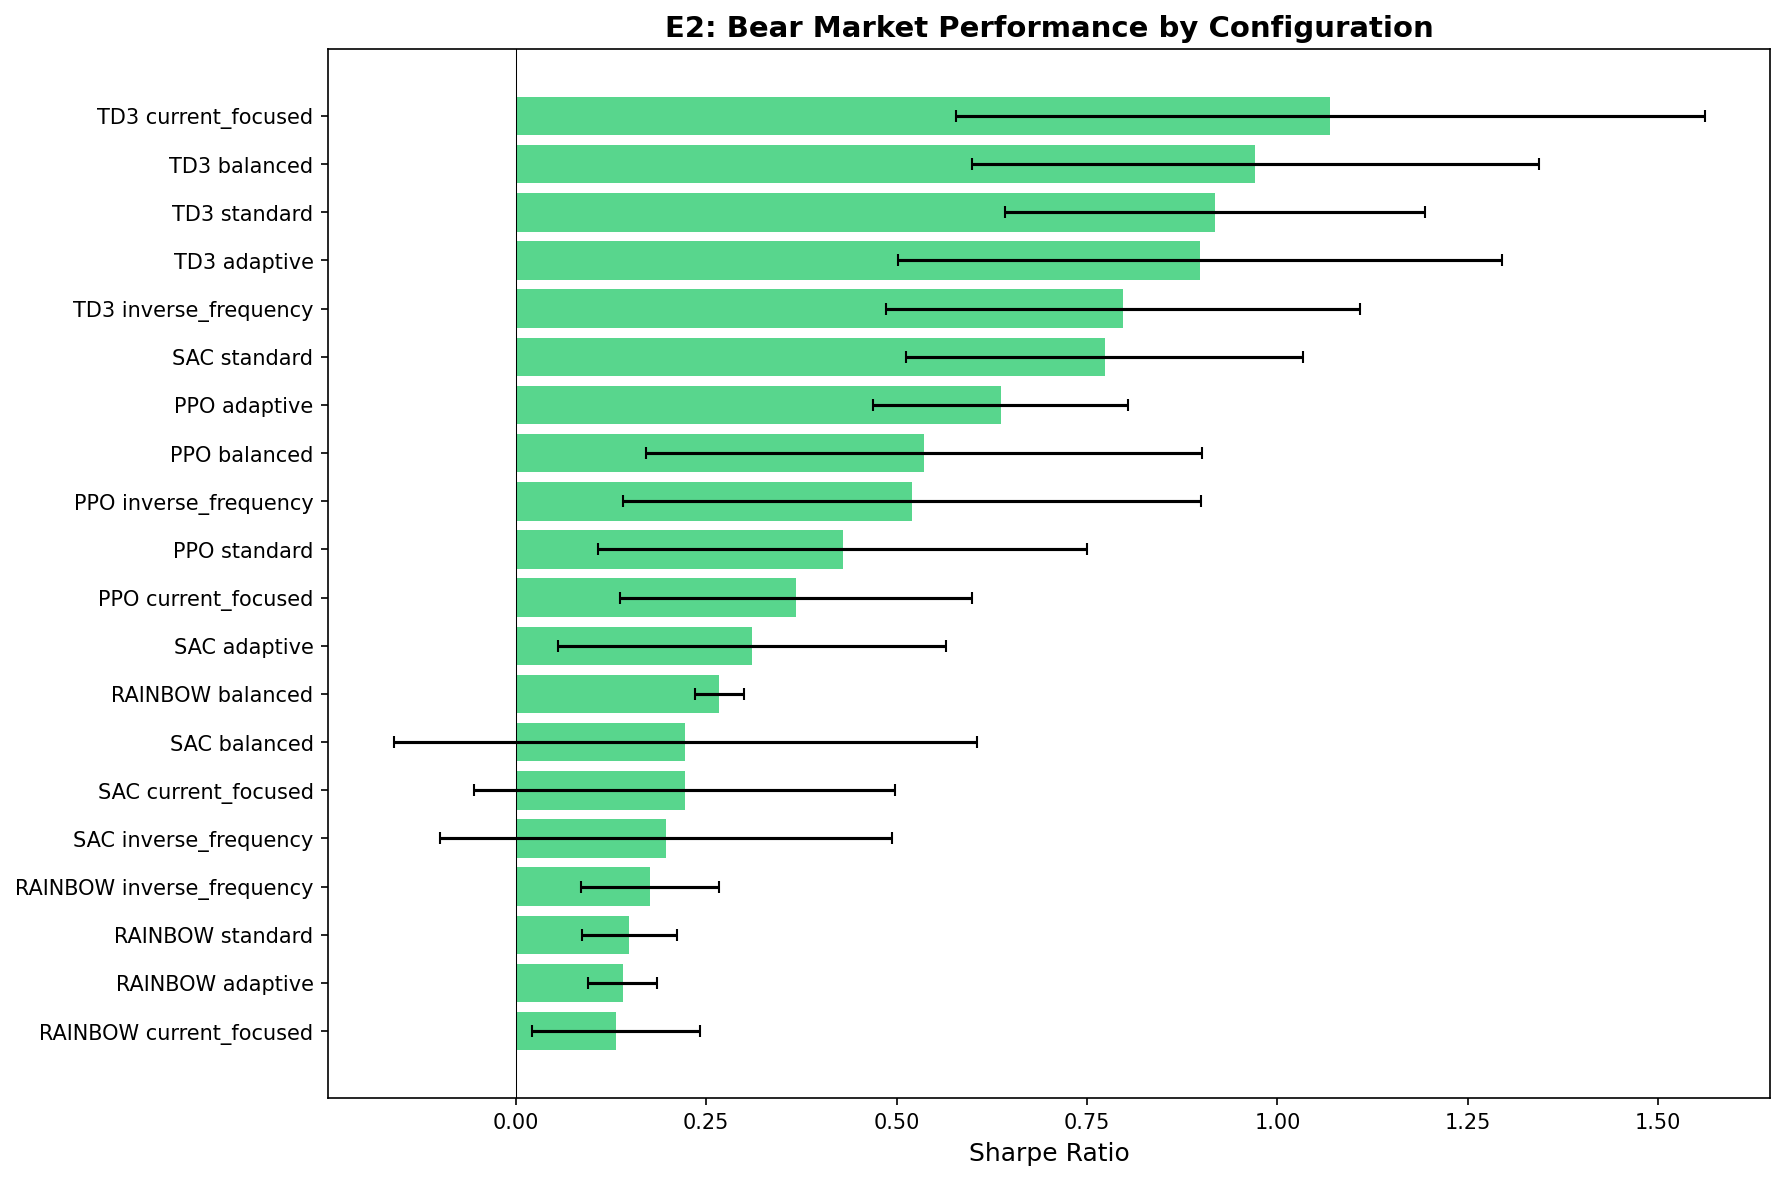
\includegraphics[width=0.88\textwidth]{figures/e2_bear_market_rankings.png}
    \caption{Bear market Sharpe ratio rankings by algorithm--strategy configuration (E2). TD3 configurations dominate the top positions, with TD3 current-focused achieving +1.069. The gap between TD3 and other algorithms is statistically significant ($p < 0.001$ for all pairwise comparisons).}
    \label{fig:app-bear-rankings}
\end{figure}

\begin{figure}[H]
    \centering
    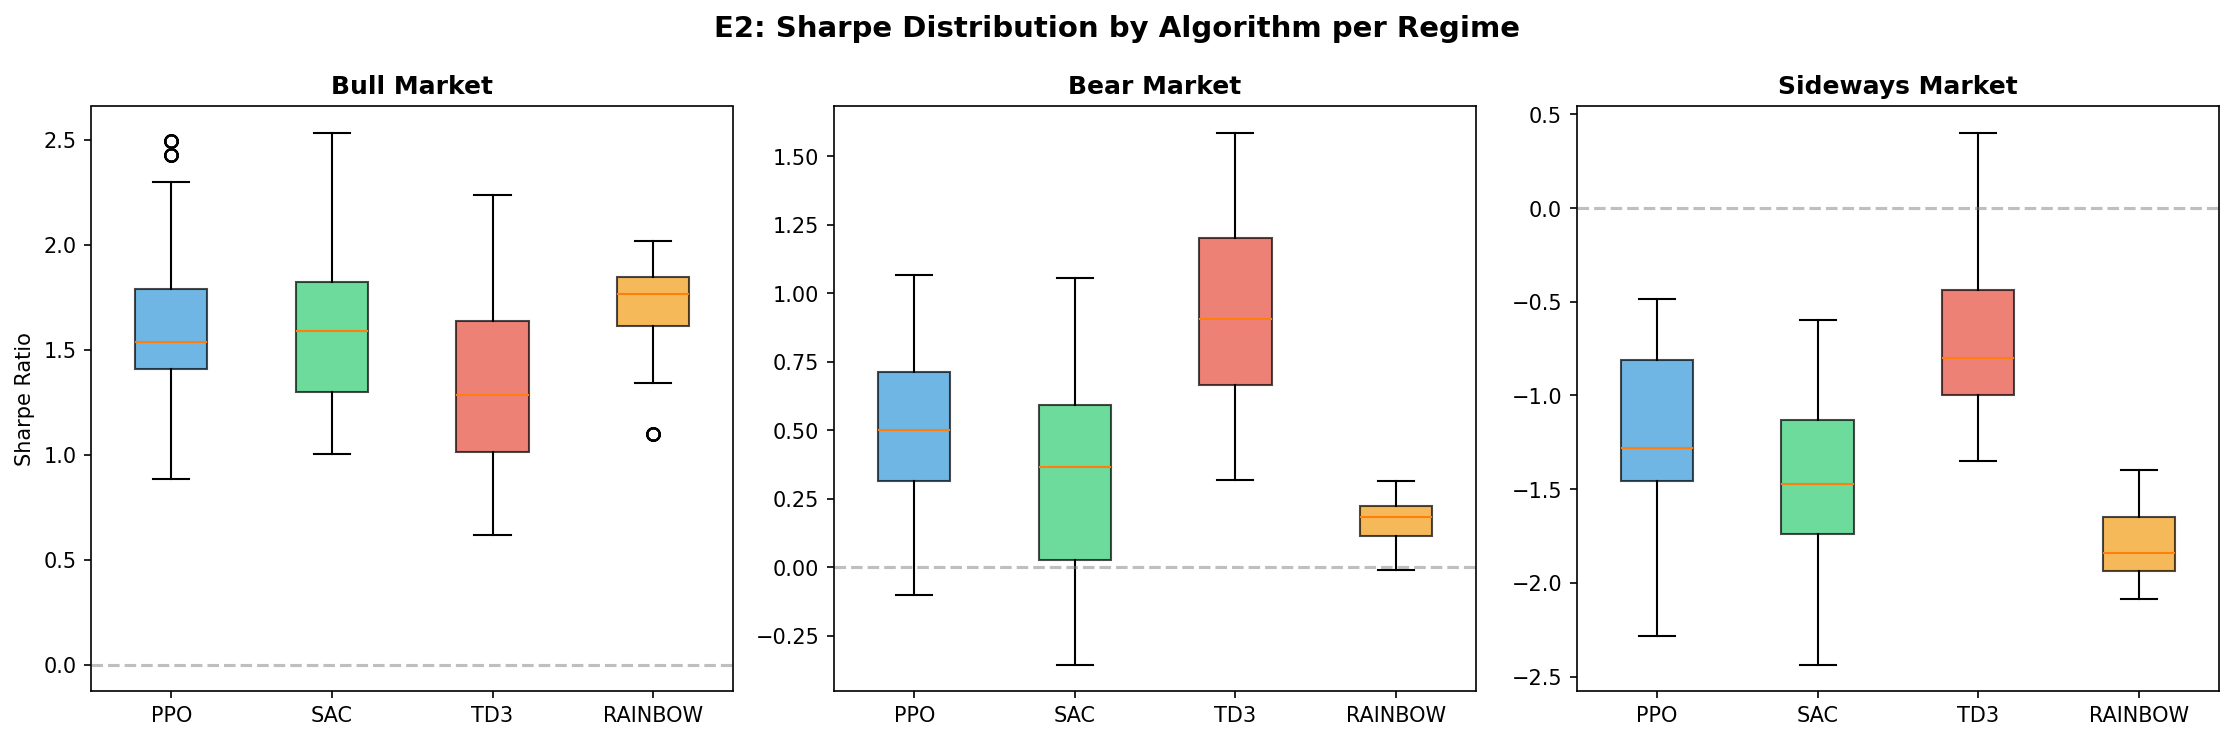
\includegraphics[width=0.88\textwidth]{figures/e2_regime_sharpe_boxplots.png}
    \caption{Distribution of Sharpe ratios by market regime across all 100 E1 runs. Bull markets show consistently positive Sharpe ratios with moderate variance. Bear markets display wider dispersion but remain predominantly positive. Sideways markets are universally challenging, with all configurations producing negative median Sharpe ratios.}
    \label{fig:app-regime-boxplots}
\end{figure}

\subsection{E3--E7: Secondary Experiments}

\begin{figure}[H]
    \centering
    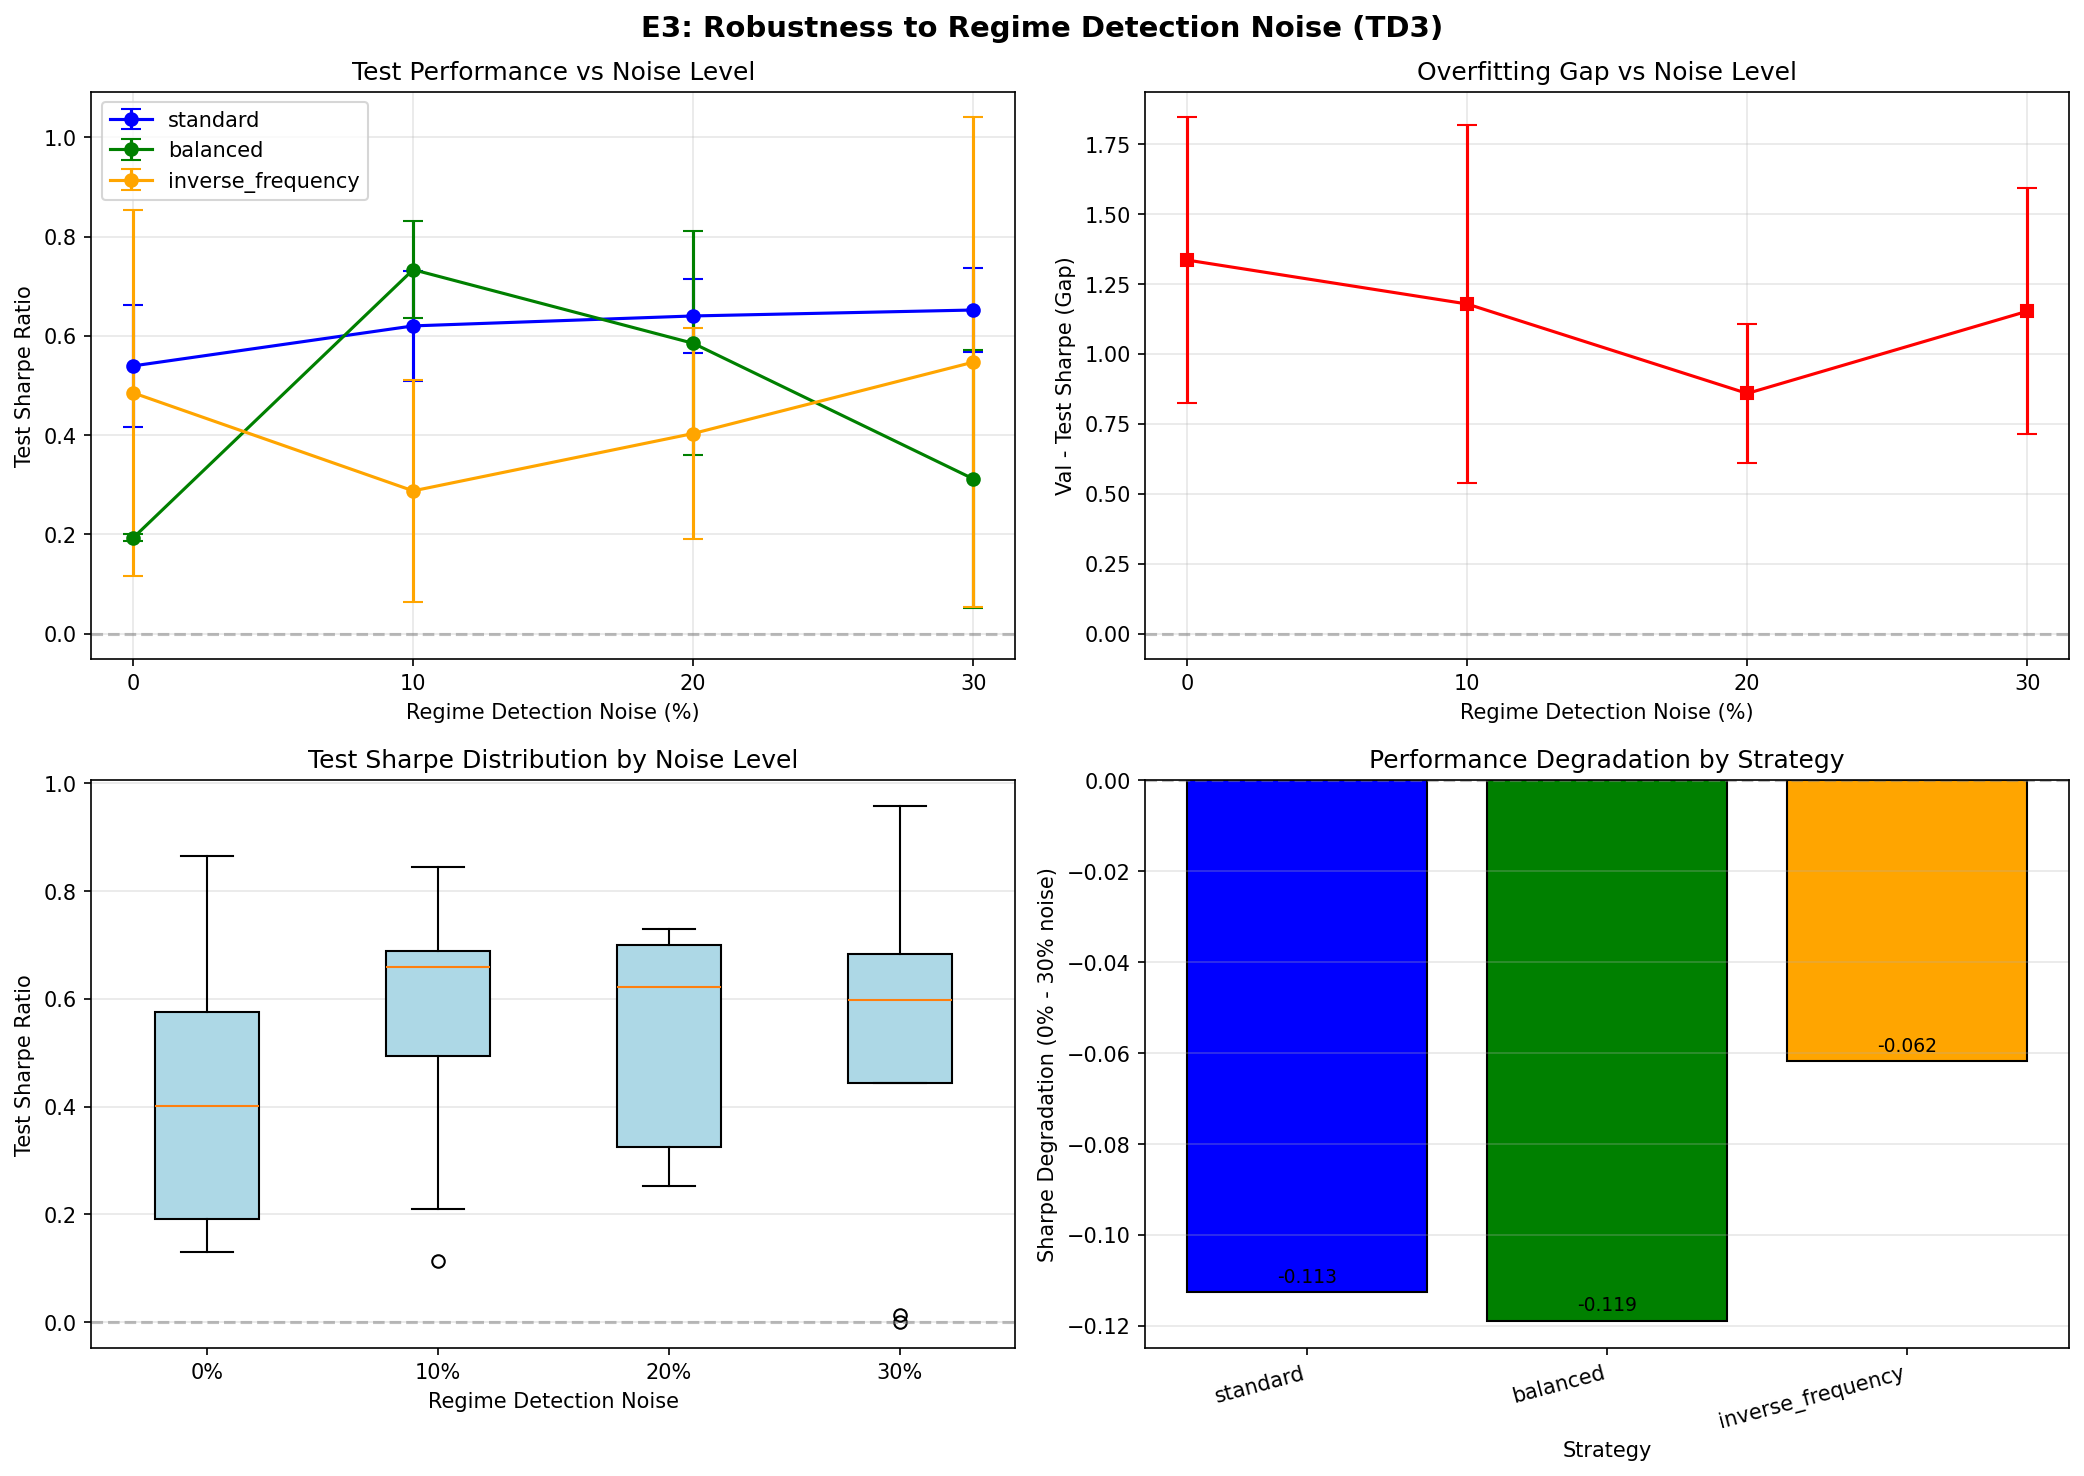
\includegraphics[width=0.88\textwidth]{figures/e3_robustness_analysis.png}
    \caption{E3 robustness to noisy regime detection (TD3, 36 runs). Four panels show the effect of increasing noise (0--30\%) on test Sharpe, validation--test gap, maximum drawdown, and strategy comparison. Standard replay is the most robust strategy, maintaining positive Sharpe ratios even at 30\% label noise. Notably, moderate noise (10--20\%) sometimes improves performance, suggesting a regularization effect.}
    \label{fig:app-e3}
\end{figure}

\begin{figure}[H]
    \centering
    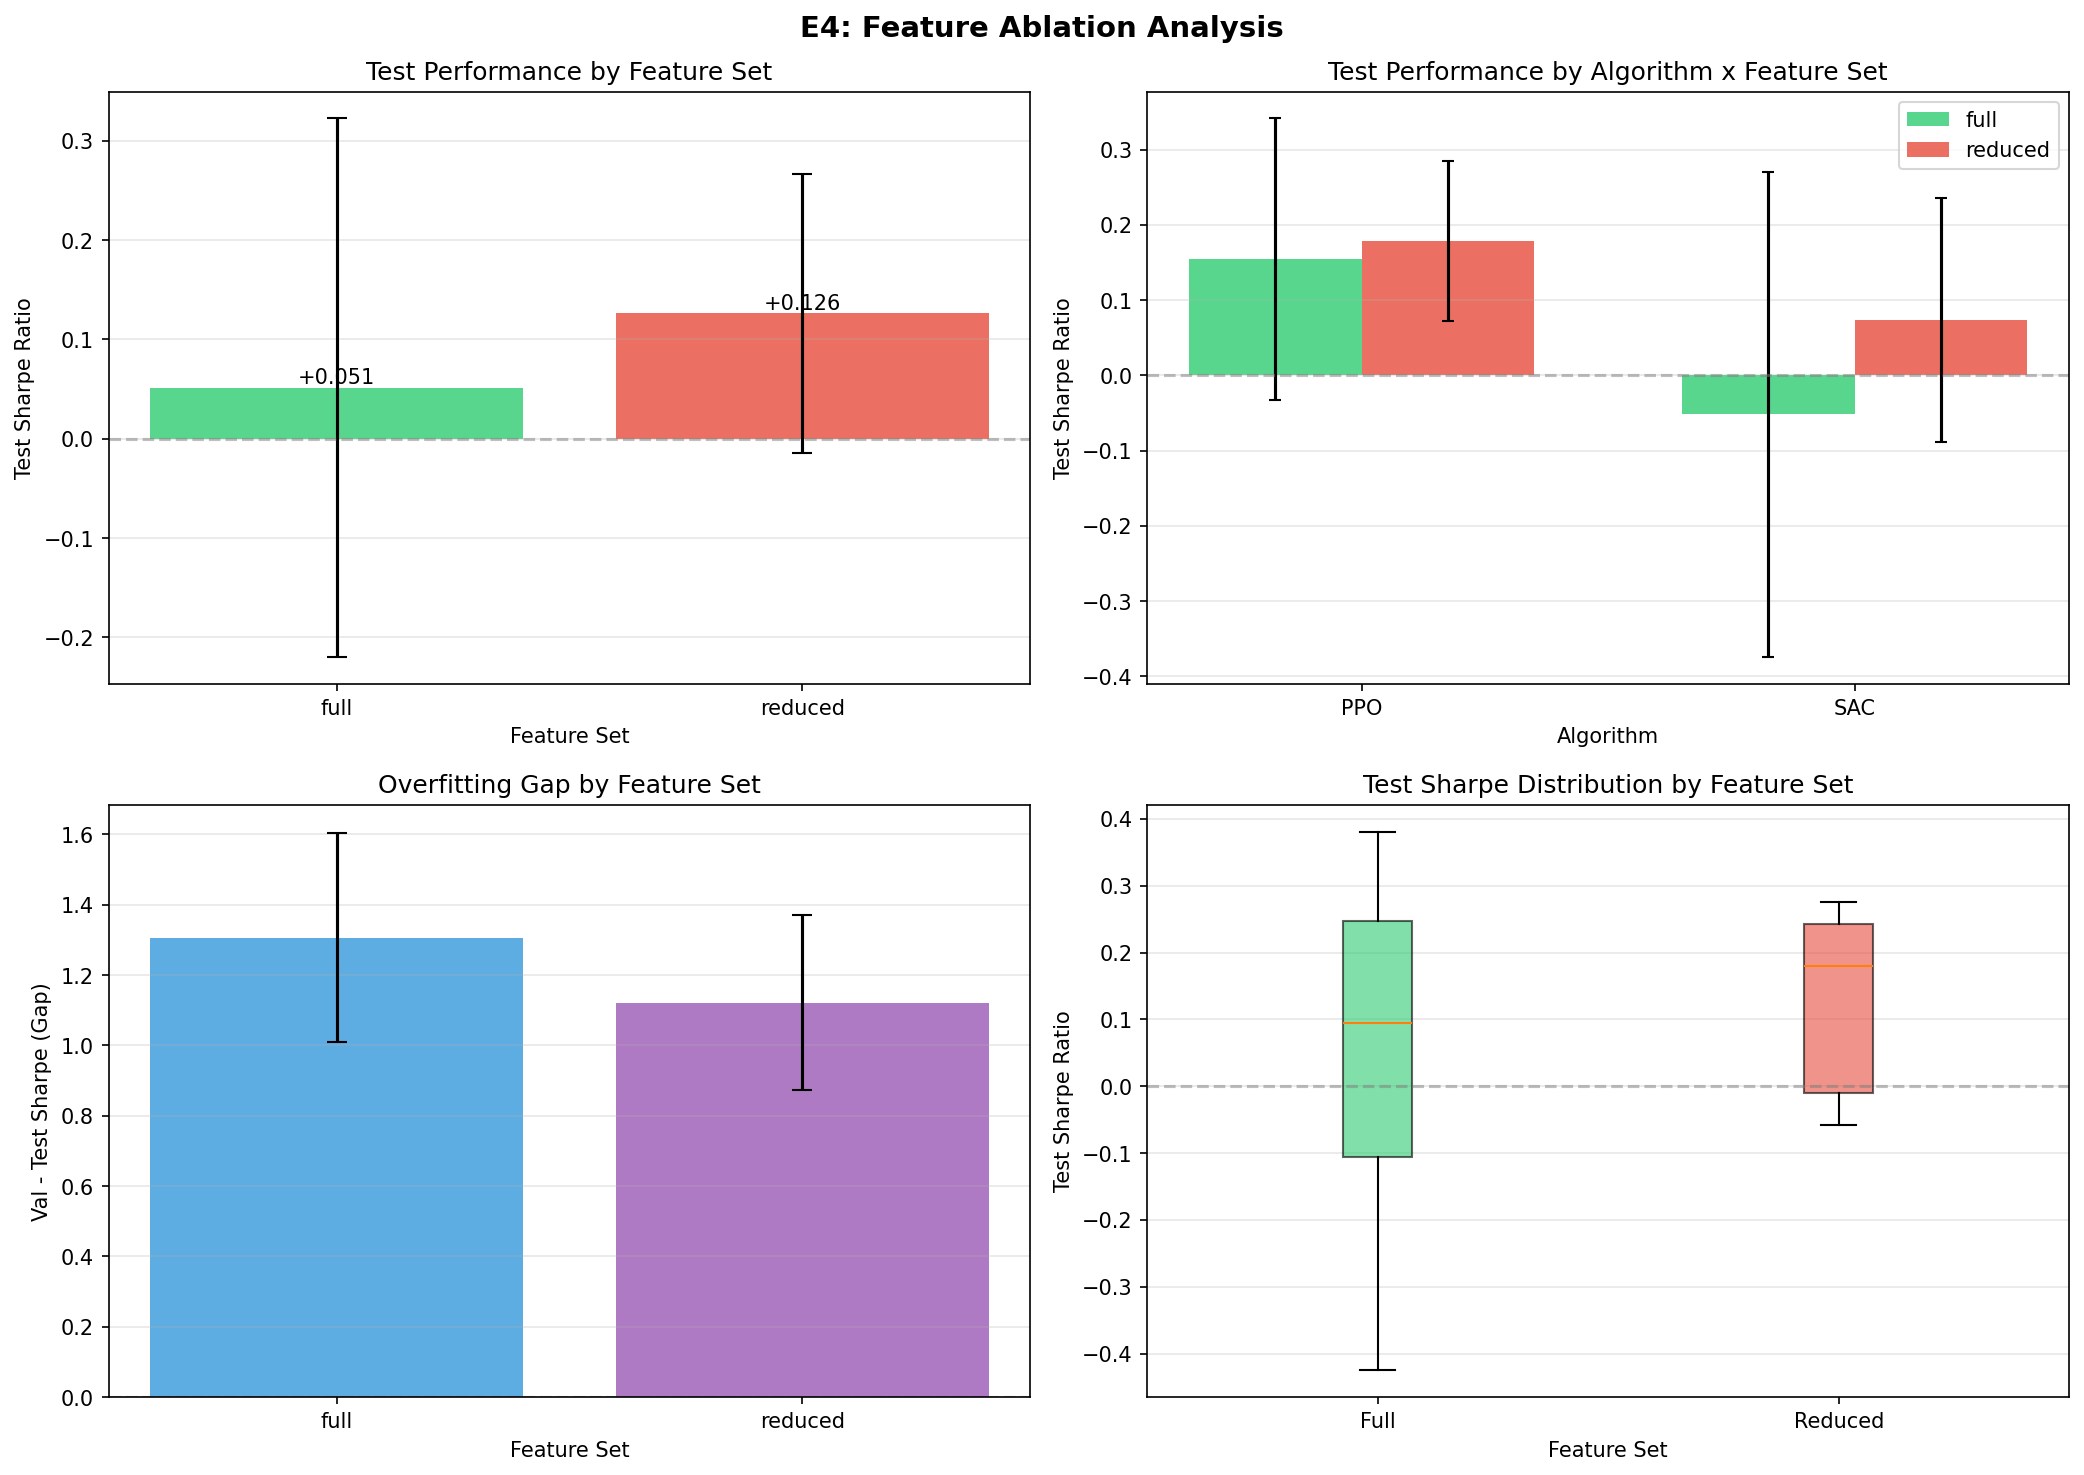
\includegraphics[width=0.88\textwidth]{figures/e4_feature_ablation.png}
    \caption{E4 feature ablation (20 runs: PPO and SAC). Comparison of full (92 features) versus reduced feature sets. Reduced features achieve comparable or slightly better test Sharpe ratios with consistently smaller validation--test gaps, suggesting that the full feature set contributes to overfitting without improving generalization.}
    \label{fig:app-e4}
\end{figure}

\begin{figure}[H]
    \centering
    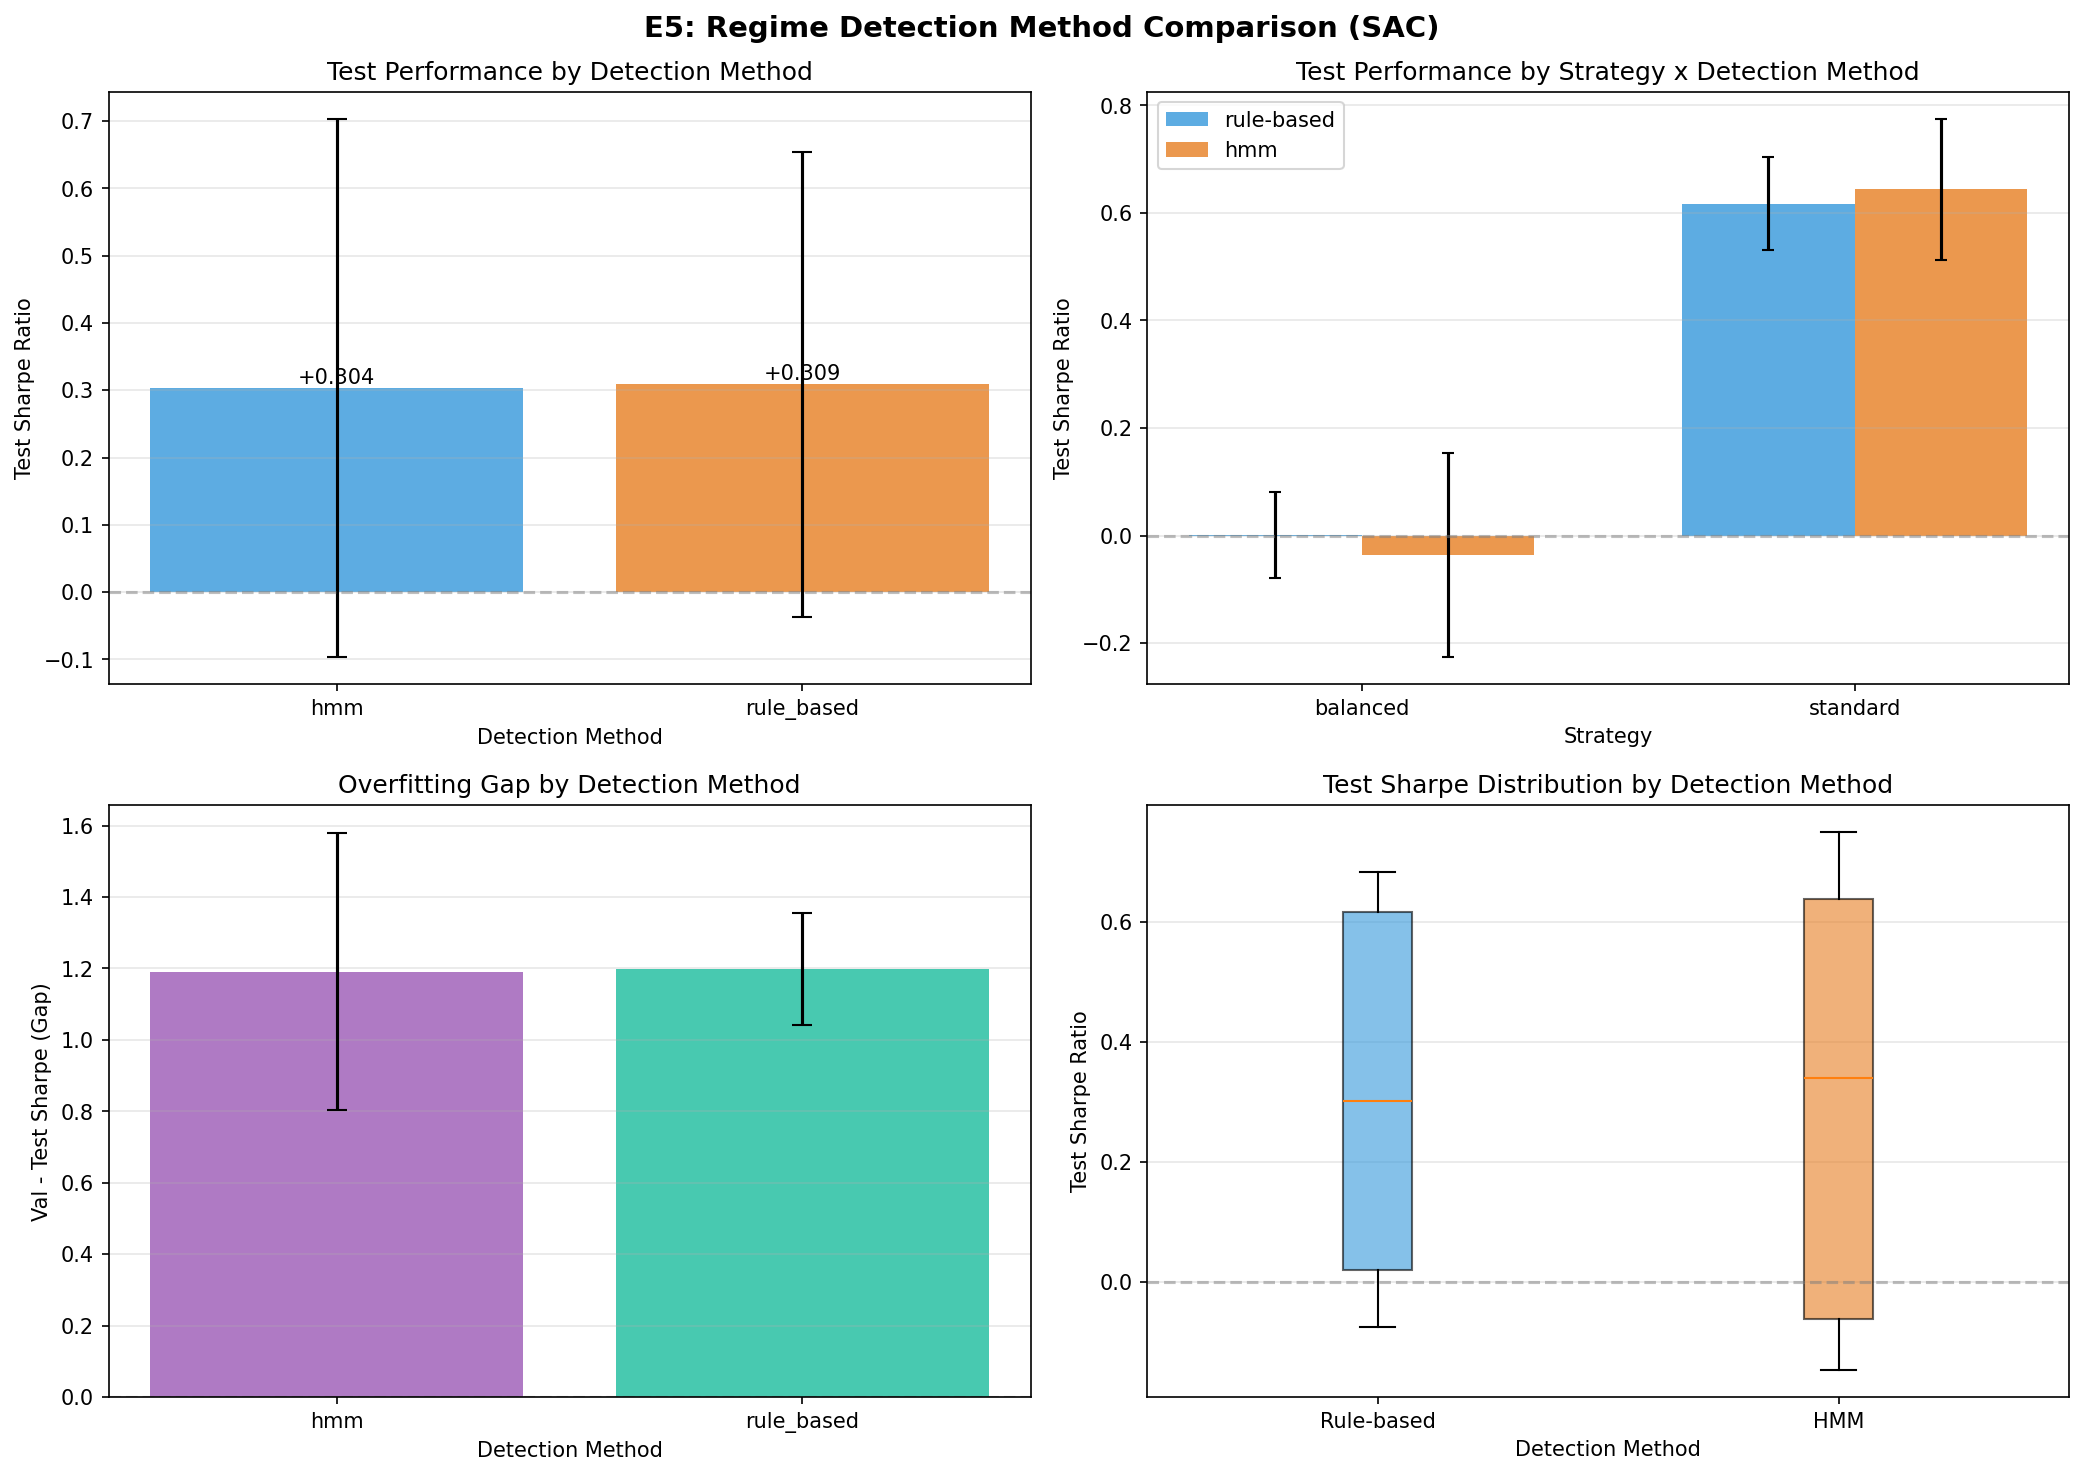
\includegraphics[width=0.88\textwidth]{figures/e5_detection_comparison.png}
    \caption{E5 regime detection method comparison (12 runs: SAC). HMM-based and rule-based detectors produce nearly identical results when using standard replay (HMM: +0.644, rule-based: +0.617). With balanced replay, both methods degrade, confirming that the SAC incompatibility is strategy-driven rather than detection-method-driven.}
    \label{fig:app-e5}
\end{figure}

\begin{figure}[H]
    \centering
    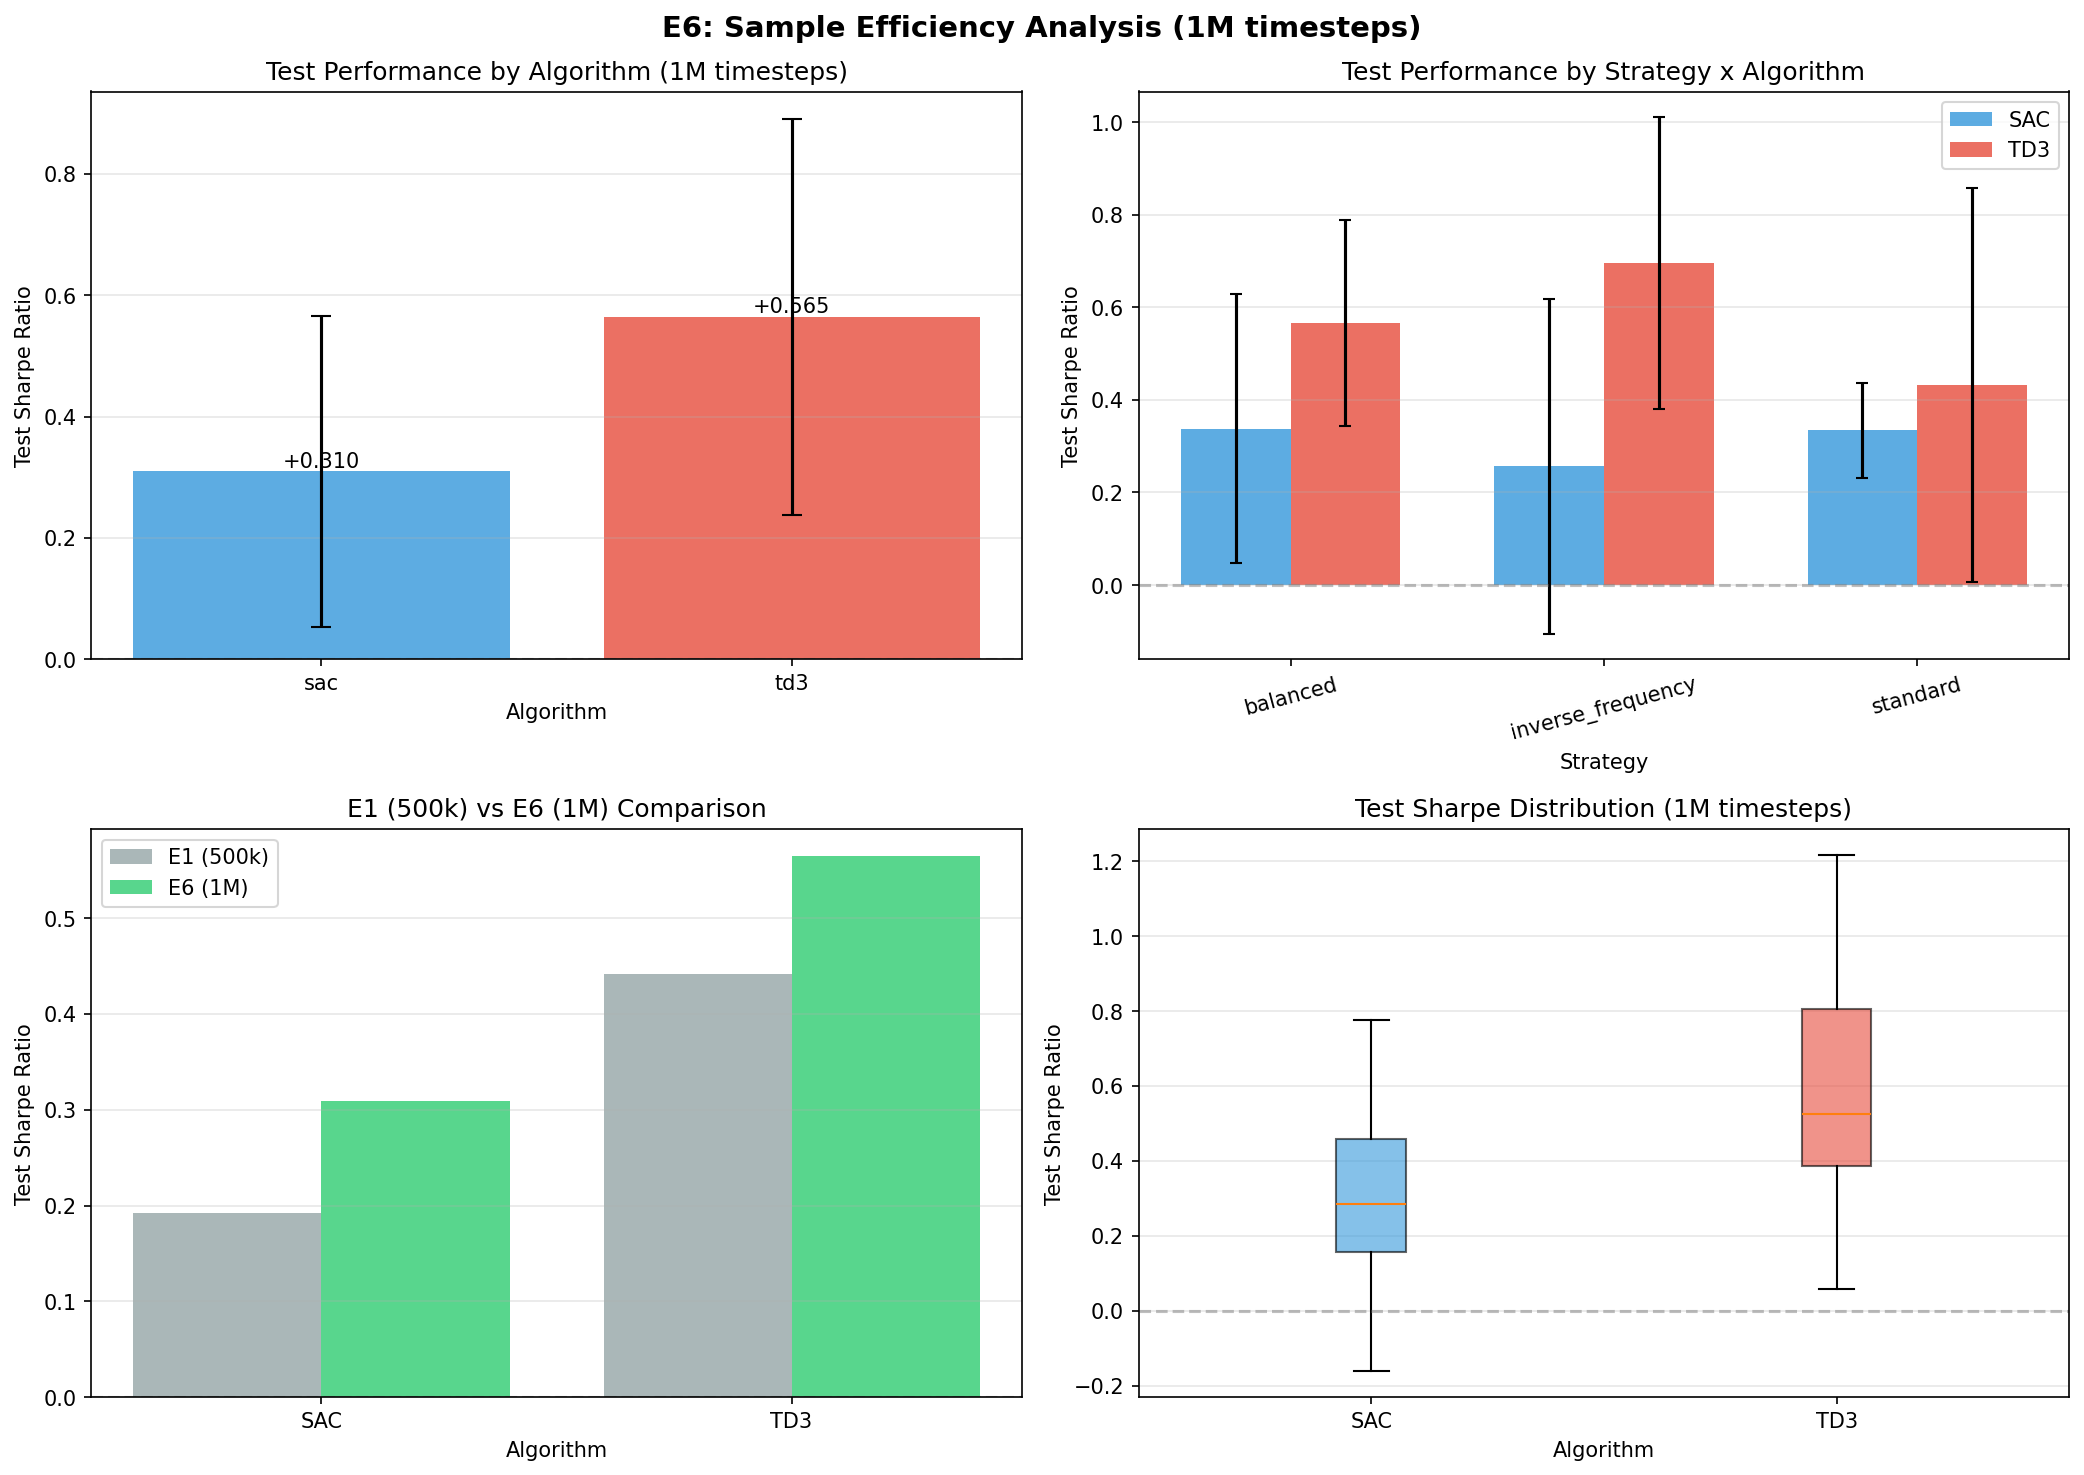
\includegraphics[width=0.88\textwidth]{figures/e6_sample_efficiency.png}
    \caption{E6 sample efficiency at 1M timesteps (30 runs: TD3 and SAC). TD3 achieves higher Sharpe ratios than SAC across all replay strategies, with TD3 inverse-frequency reaching +0.695. Extended training beyond 500k timesteps provides diminishing returns for both algorithms.}
    \label{fig:app-e6}
\end{figure}

\begin{figure}[H]
    \centering
    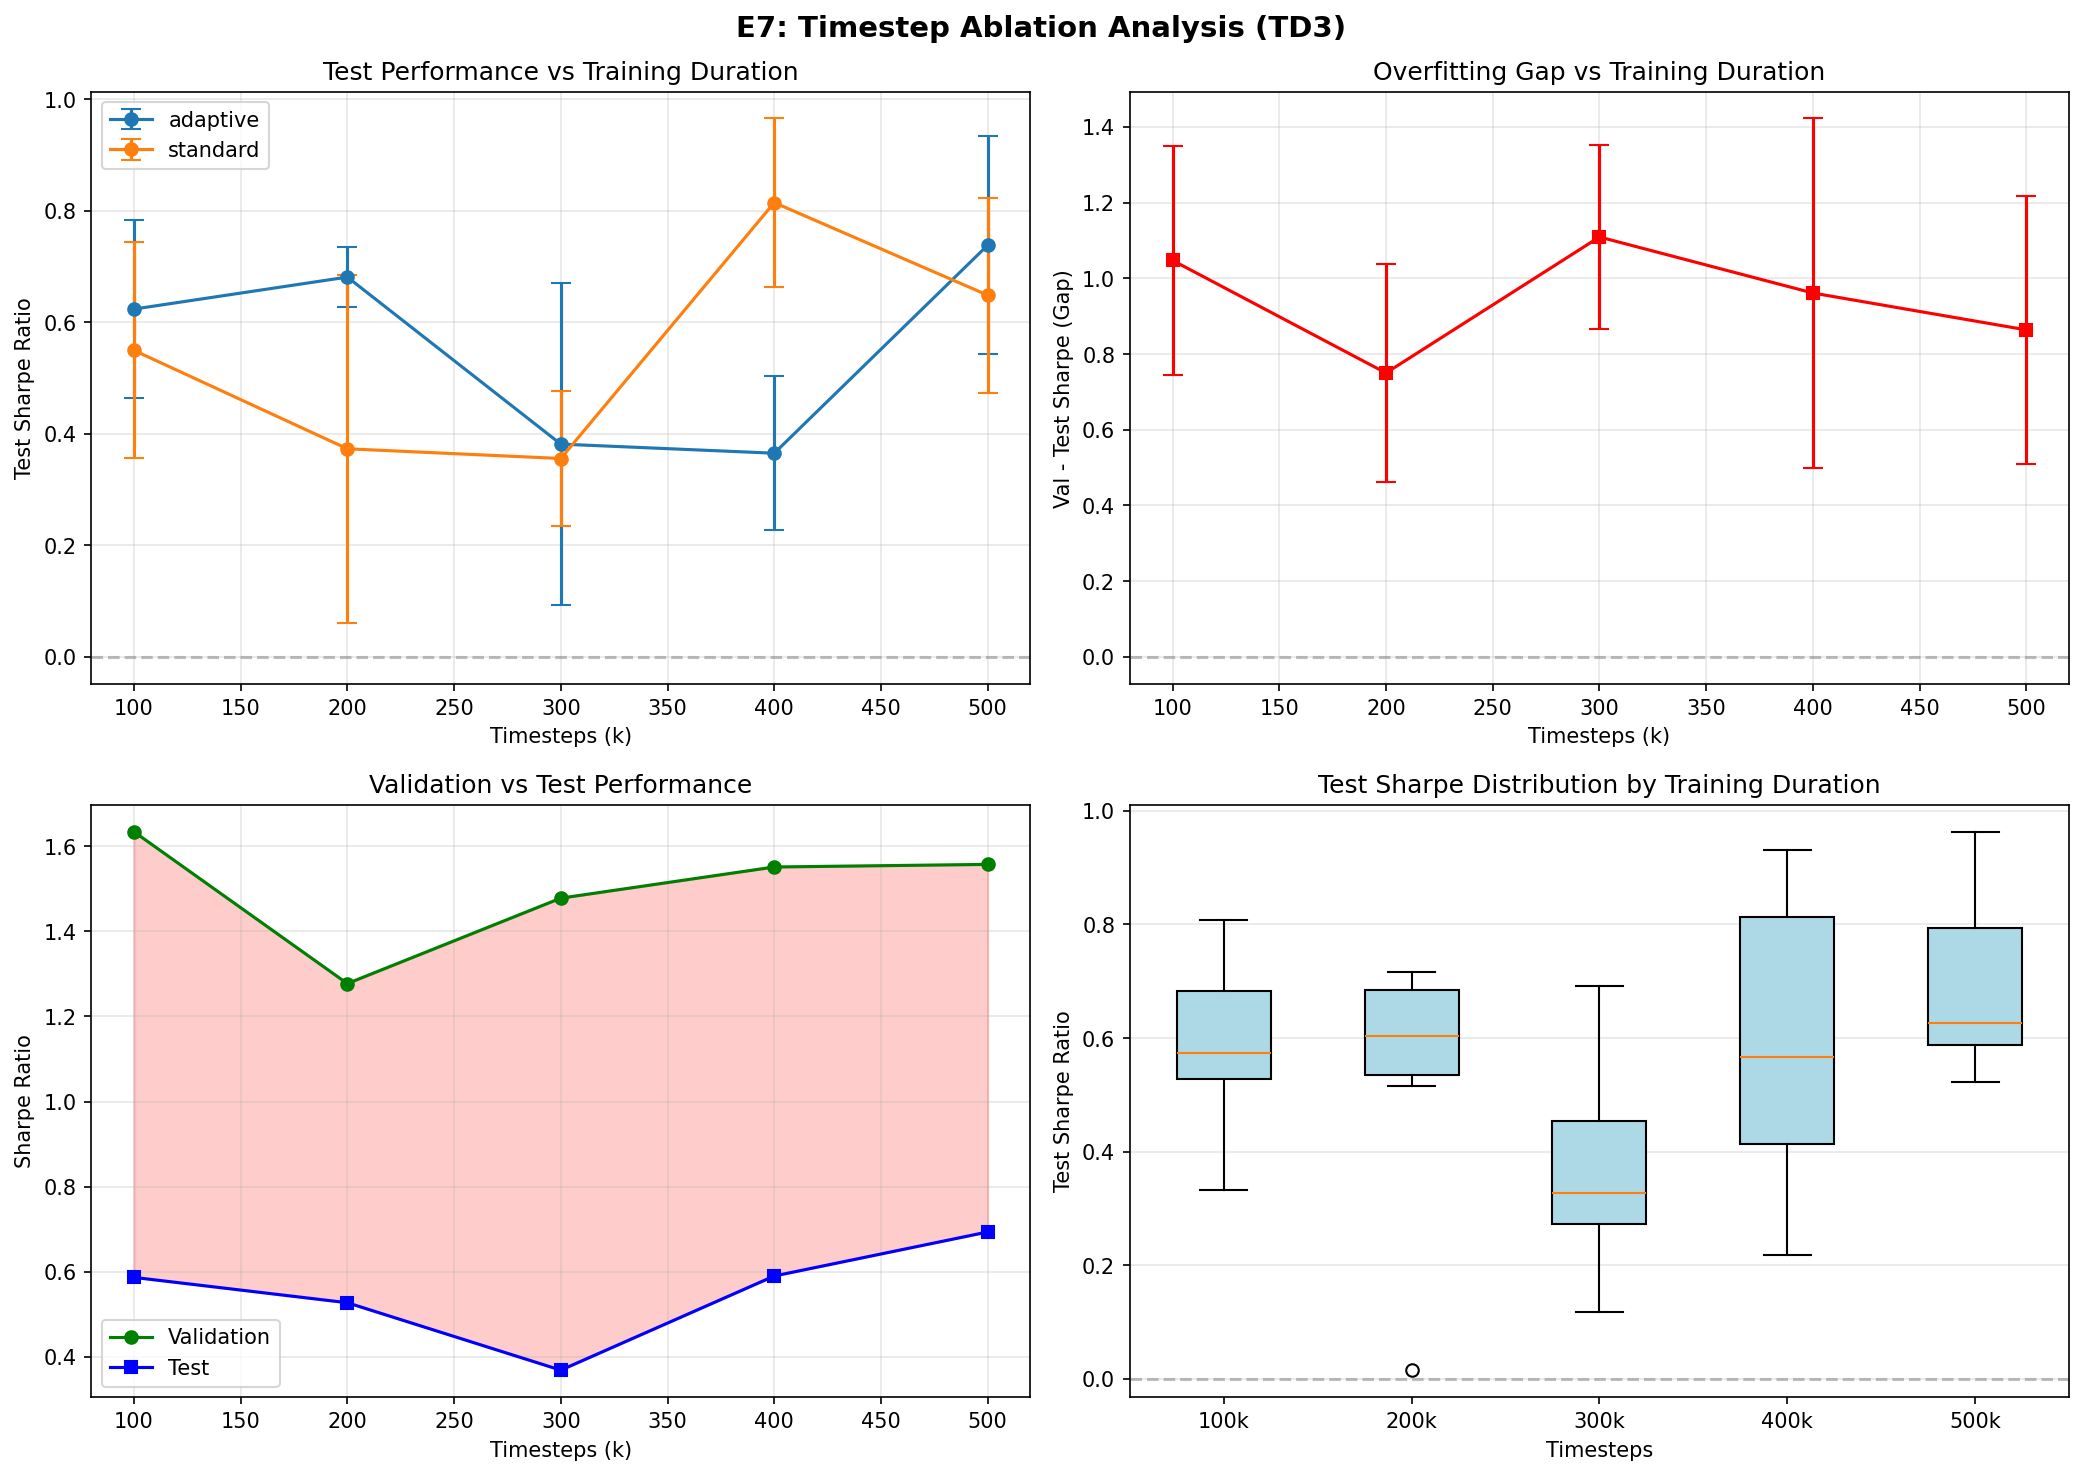
\includegraphics[width=0.88\textwidth]{figures/e7_timestep_analysis.png}
    \caption{E7 timestep ablation for TD3 (30 runs). Test Sharpe and validation--test gap as a function of training duration (100k--500k timesteps). The optimal point is 400k timesteps with standard replay, which achieves both the highest test Sharpe (+0.815) and the lowest validation--test gap (0.607). Training beyond 400k leads to mild overfitting, as evidenced by increasing gaps without corresponding test improvements.}
    \label{fig:app-e7}
\end{figure}

\subsection{Context and Baselines}

\begin{figure}[H]
    \centering
    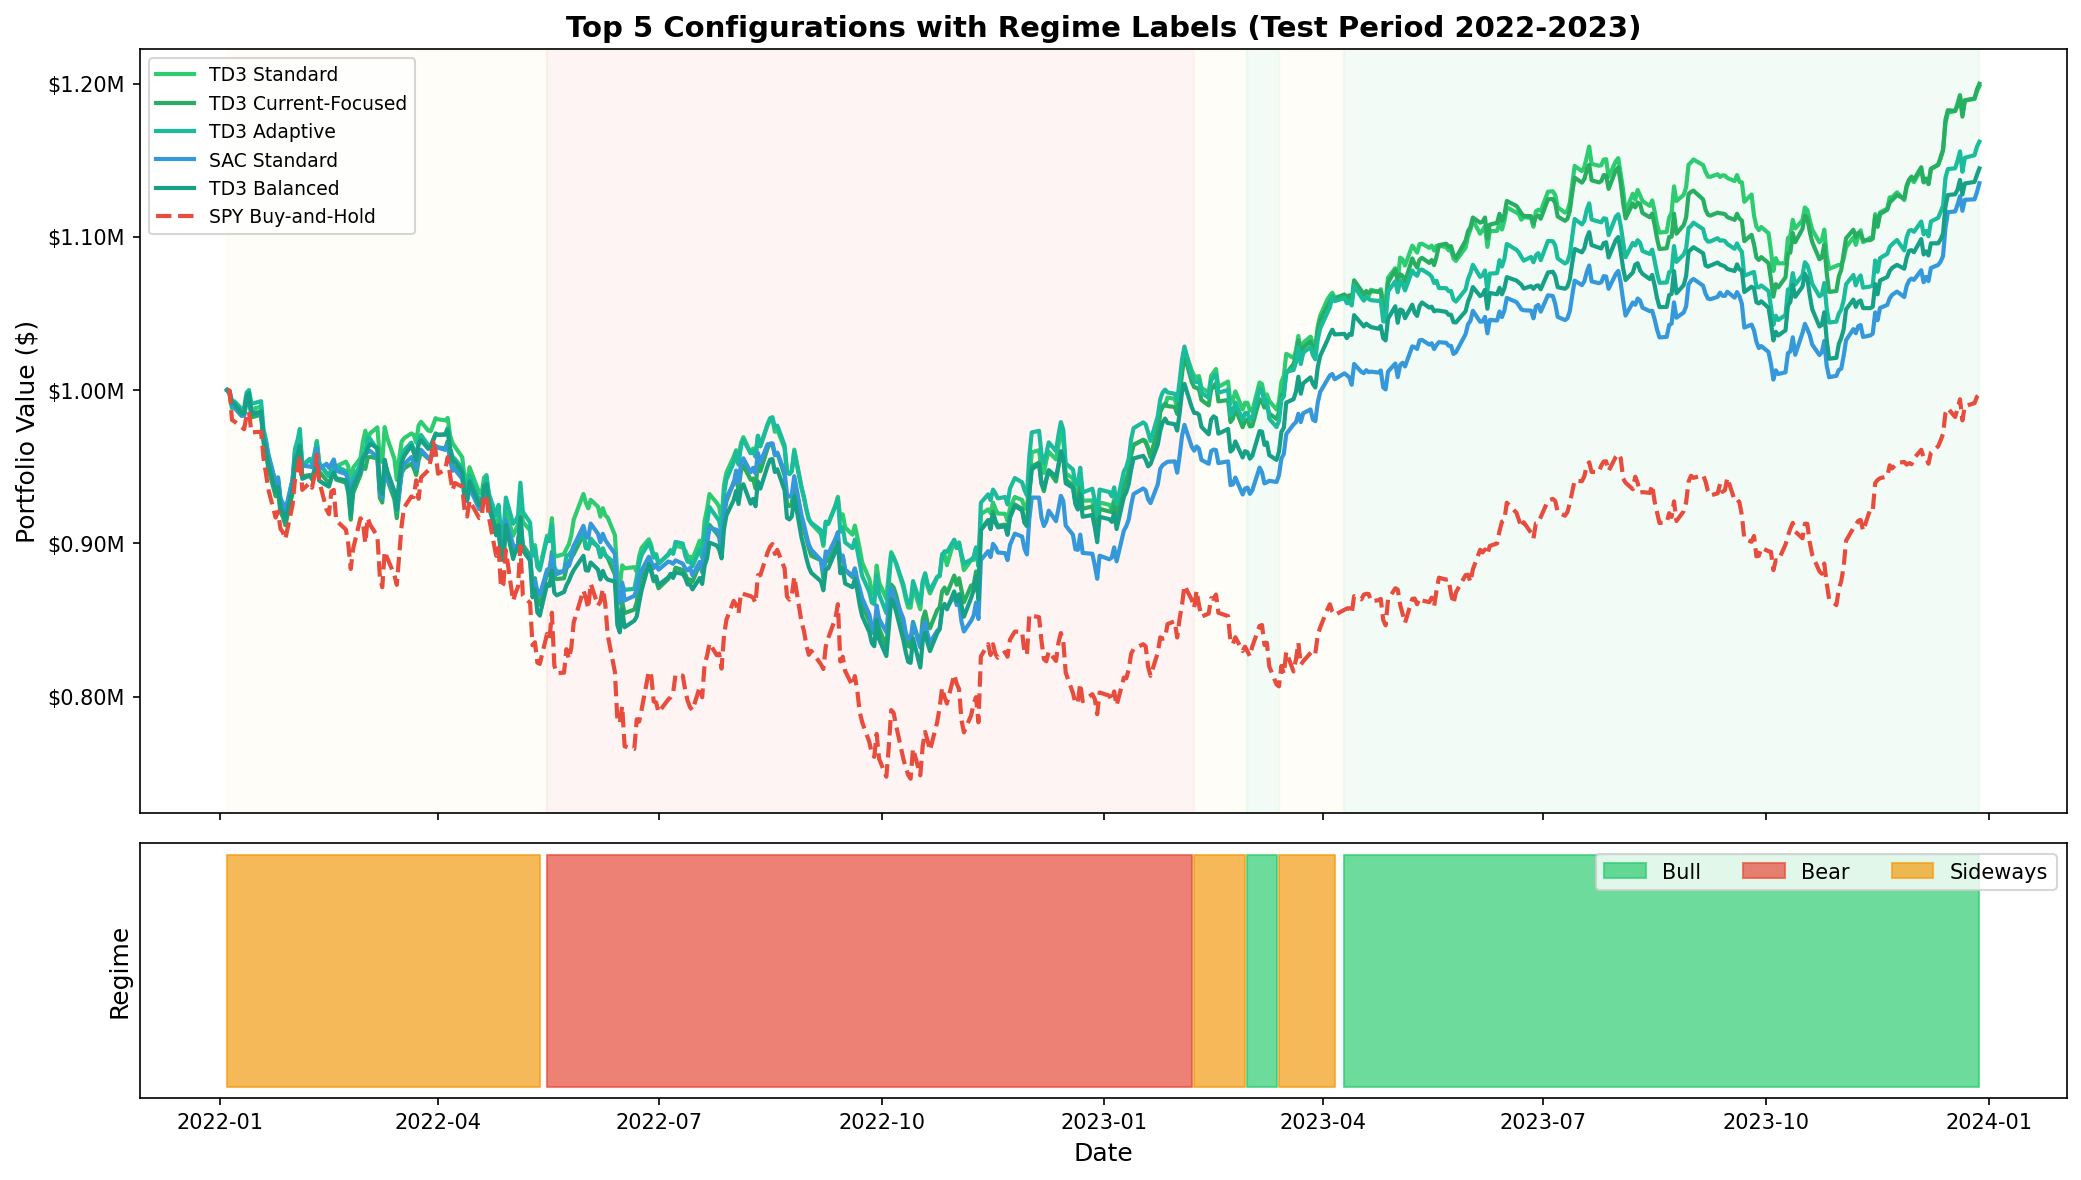
\includegraphics[width=0.88\textwidth]{figures/regime_timeline.png}
    \caption{Portfolio value trajectories for the top 5 configurations with market regime shading (bull in green, bear in red, sideways in yellow) over the 2022--2023 test period. The regime detector identifies the 2022 bear market and the 2023 recovery, which the RL agents exploit by adjusting portfolio allocation.}
    \label{fig:app-regime-timeline}
\end{figure}

\begin{figure}[H]
    \centering
    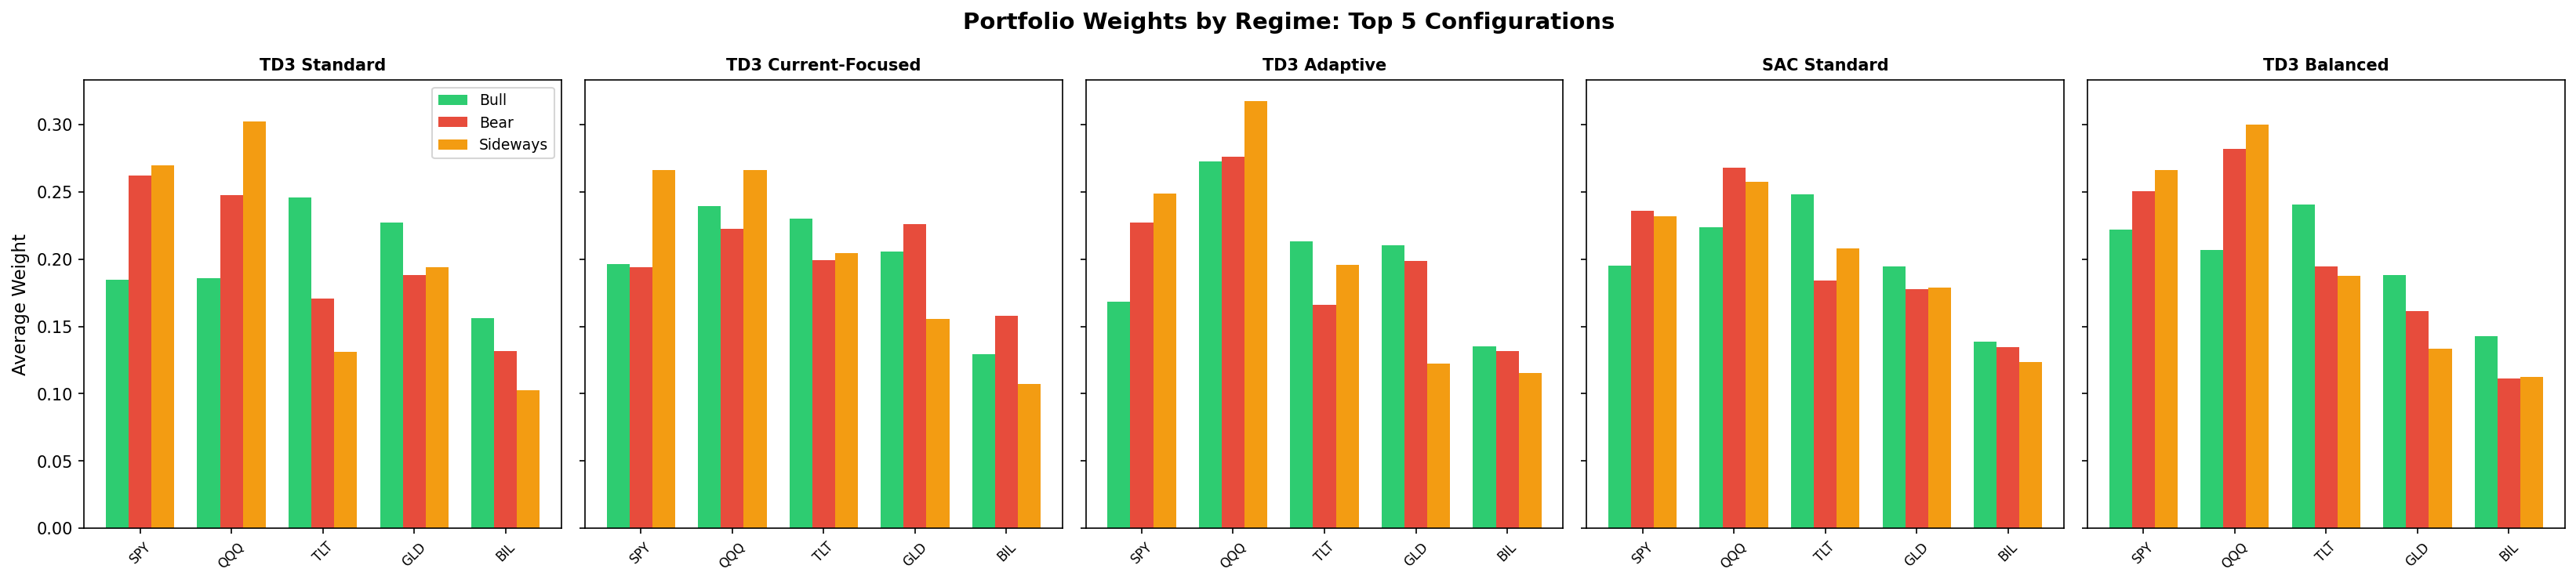
\includegraphics[width=0.75\textwidth]{figures/weights_by_regime.png}
    \caption{Mean portfolio weights by market regime for the top 5 configurations. Counter-intuitively, agents allocate more to risk assets (SPY+QQQ) during bear markets than during bull markets, suggesting exploitation of mean-reversion opportunities within bear-market rallies.}
    \label{fig:app-weights-regime}
\end{figure}

\begin{figure}[H]
    \centering
    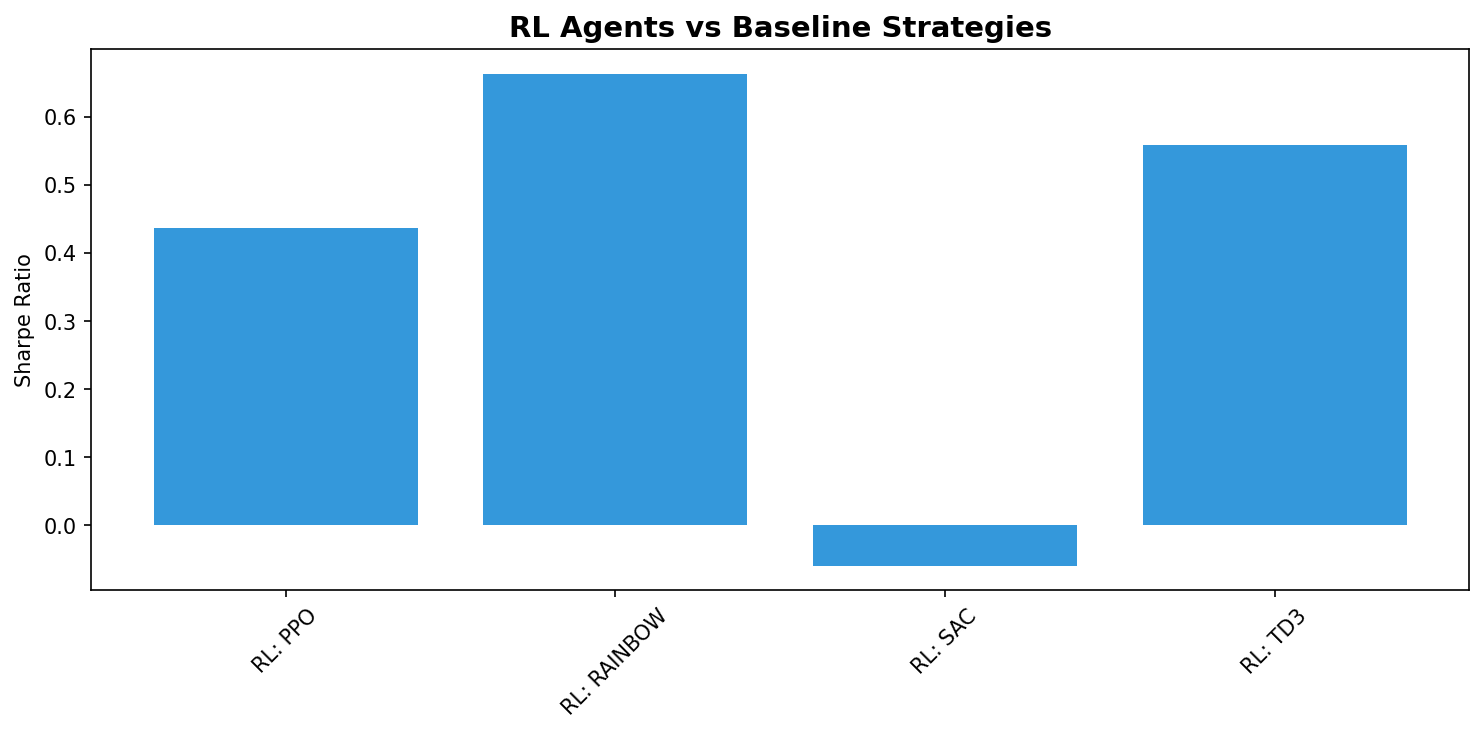
\includegraphics[width=0.75\textwidth]{figures/baseline_comparison.png}
    \caption{Test Sharpe ratios for passive baselines and top RL configurations. All four baselines produce negative or near-zero Sharpe ratios during the 2022--2023 period, while RL agents---particularly TD3---achieve substantially positive risk-adjusted returns.}
    \label{fig:app-baselines}
\end{figure}


\section{Implementation Details}
\label{app:implementation}

This appendix provides key code excerpts from the regime-aware replay buffer, the core novel component of our system.

\subsection{Regime-Aware Replay Buffer: Sampling Strategies}

The \texttt{RegimeAwareReplayBuffer} partitions experiences by regime and samples according to a configurable strategy. The \texttt{sample()} method dispatches to strategy-specific implementations:

\begin{lstlisting}[caption={Main sampling dispatcher},label={lst:sample-dispatch}]
def sample(self, batch_size, current_regime=None):
    if self.strategy == SamplingStrategy.BALANCED:
        return self._sample_balanced(batch_size)
    elif self.strategy == SamplingStrategy.CURRENT_FOCUSED:
        return self._sample_current_focused(batch_size, current_regime)
    elif self.strategy == SamplingStrategy.INVERSE_FREQUENCY:
        return self._sample_inverse_frequency(batch_size)
    elif self.strategy == SamplingStrategy.ADAPTIVE:
        return self._sample_adaptive(batch_size)
\end{lstlisting}

\subsubsection{Balanced Sampling}
Draws equal numbers from each regime buffer, with fallback redistribution when a regime has fewer samples than requested:

\begin{lstlisting}[caption={Balanced sampling implementation},label={lst:balanced}]
def _sample_balanced(self, batch_size):
    available = {r: len(buf) for r, buf in self._regime_buffers.items()}
    base_per_regime = batch_size // len(MarketRegime)  # 3 regimes

    samples_per_regime = {}
    remaining = batch_size
    for regime in MarketRegime:
        n = min(base_per_regime, available[regime])
        samples_per_regime[regime] = n
        remaining -= n

    # Distribute remaining to regimes with extras
    for regime in shuffled(MarketRegime):
        if remaining <= 0: break
        extra = min(remaining, available[regime] - samples_per_regime[regime])
        samples_per_regime[regime] += extra
        remaining -= extra

    # Sample indices from each regime buffer
    for regime, n in samples_per_regime.items():
        indices = np.random.choice(len(buf), n, replace=False)
        experiences.extend([buf[i] for i in indices])
\end{lstlisting}

\subsubsection{Inverse-Frequency Sampling}
Oversamples rare regimes by weighting inversely to buffer size:

\begin{lstlisting}[caption={Inverse-frequency sampling},label={lst:inverse-freq}]
def _sample_inverse_frequency(self, batch_size):
    counts = {r: len(buf) for r, buf in self._regime_buffers.items()}
    weights = {r: 1.0 / (count + 1) for r, count in counts.items()}
    total_weight = sum(weights.values())
    proportions = {r: w / total_weight for r, w in weights.items()}
    # Sample batch_size * proportions[r] from each regime
\end{lstlisting}

\subsubsection{Adaptive Sampling with TD Error Tracking}
Samples proportionally to mean TD error per regime, using EMA decay:

\begin{lstlisting}[caption={Adaptive sampling and TD error update},label={lst:adaptive}]
def _sample_adaptive(self, batch_size):
    mean_td = {r: self._td_errors_sum[r] / max(self._td_errors_count[r], 1)
               for r in MarketRegime}
    total_td = sum(mean_td.values())
    if total_td <= 0:
        return self._sample_balanced(batch_size)  # fallback
    proportions = {r: td / total_td for r, td in mean_td.items()}
    # Sample batch_size * proportions[r] from each regime

def update_td_errors(self, regime, td_errors):
    """Update TD error stats using EMA (decay=0.99)."""
    decay = self._td_ema_decay  # 0.99
    self._td_errors_sum[regime] = (
        decay * self._td_errors_sum[regime] + np.sum(np.abs(td_errors))
    )
    self._td_errors_count[regime] = (
        decay * self._td_errors_count[regime] + len(td_errors)
    )
\end{lstlisting}



\section{Bug Fix Documentation}
\label{app:bugs}

During development, we identified and fixed eleven bugs that significantly impacted experimental results. Nine were corrected before initial execution; two additional bugs (\#10, \#11) were discovered post-execution, and affected experiments were re-run. This documentation demonstrates the engineering rigor applied to ensure correct metric calculation.

\begin{table}[H]
\centering
\caption{Bug Fixes Applied}
\label{tab:bugs}
\begin{tabular}{clp{6cm}l}
\toprule
\textbf{\#} & \textbf{Bug} & \textbf{Impact} & \textbf{File} \\
\midrule
1 & Episode length (val/test) & Incorrect episode termination & experiment\_runner.py \\
2 & Rainbow regime\_detector & Missing regime detector & rainbow\_agent.py \\
3 & agent\_factory regime\_detector & Missing parameter passing & agent\_factory.py \\
4 & E3 SAC$\to$TD3 & Wrong algorithm for robustness & run\_config.py \\
5 & Transaction cost double-count & Costs subtracted twice & trading\_env.py \\
6 & Cumulative return compounding & Incorrect return calculation & experiment\_runner.py \\
7 & Test/Val date mismatch & Wrong date ranges & experiment\_runner.py \\
8 & N\_EVAL\_EPISODES mismatch & Inconsistent episode counts & experiment\_runner.py \\
9 & Adaptive TD error accumulation & TD errors accumulated without decay & regime\_aware\_buffer.py \\
10 & Bug \#9 incomplete: \texttt{add()} & \texttt{add()} still accumulated TD errors without EMA & regime\_aware\_buffer.py \\
11 & Risk parity look-ahead bias & \texttt{iloc[-60:]} used future data & compute\_baselines.py \\
\bottomrule
\end{tabular}
\end{table}

The most impactful bugs were \#5 (transaction cost double-counting), which inflated cost penalties by subtracting transaction costs in both the reward calculation and the portfolio value update, and \#6 (cumulative return compounding), which summed step returns instead of compounding portfolio values, causing significant metric errors over 252-step episodes. Bug \#9 (adaptive TD error accumulation) caused TD error sums to grow unboundedly, eventually making all regimes appear equally important and collapsing the adaptive strategy to uniform sampling; this was fixed by introducing EMA decay ($\alpha = 0.99$). Bugs \#1--\#9 were fixed and all experiments re-executed from scratch.

Bug \#10 was discovered post-execution: the \texttt{add()} method in the replay buffer still accumulated TD errors without EMA decay, partially undoing the Bug \#9 fix. After correction, TD3 adaptive dropped from Sharpe +0.733 to +0.501. Bug \#11 fixed a look-ahead bias in the risk parity baseline (\texttt{iloc[-60:]} $\to$ \texttt{iloc[:60]}), changing its Sharpe from +0.003 to $-$0.055. E1 and E7 adaptive configurations were re-run after these fixes.


\section{Data Description}
\label{app:data}

Table~\ref{tab:assets} summarises the five ETFs used in this study. The universe spans US equities, government bonds, commodities, and cash equivalents, enabling the agent to construct diversified portfolios across market conditions.

\begin{table}[H]
\centering
\caption{Asset universe.}
\label{tab:assets}
\begin{tabular}{lll}
\toprule
Ticker & Name & Asset Class \\
\midrule
SPY & SPDR S\&P 500 ETF Trust & US Large-Cap Equity \\
QQQ & Invesco QQQ Trust (NASDAQ-100) & US Tech/Growth Equity \\
TLT & iShares 20+ Year Treasury Bond ETF & US Government Bonds \\
GLD & SPDR Gold Shares & Commodities (Gold) \\
BIL & SPDR Bloomberg 1--3 Month T-Bill ETF & Cash / Money Market \\
\bottomrule
\end{tabular}
\end{table}

Daily OHLCV (Open, High, Low, Close, Adjusted Close, Volume) data was obtained from Yahoo Finance via the \texttt{yfinance} Python library, covering 2010-01-01 to 2023-12-31 (approximately 3,500 trading days). The data was split chronologically to prevent look-ahead bias: training on 2010--2019 (approximately 2,515 days), validation on 2020--2021 (approximately 503 days), and testing on 2022--2023 (approximately 499 days). Each evaluation episode spans one full year (252 trading days) with \$1M initial capital.

The observation vector consists of 98 dimensions for off-policy algorithms (SAC, TD3, Rainbow) and 101 dimensions for PPO (which receives an additional 3-dimensional one-hot regime indicator). The base observation comprises 92 technical features plus 6 portfolio state variables (5 current weights and normalised portfolio value). Each asset receives 19 per-asset features, except SPY which receives 16 (relative strength is not computed for the benchmark asset against itself), giving a total of $16 + (4 \times 19) = 92$ market features. Table~\ref{tab:features} lists all per-asset features.

\begin{table}[H]
\centering
\small
\caption{Per-asset feature vector (19 features per asset, 16 for SPY). Features marked with $\dagger$ are excluded for SPY as relative strength cannot be computed for the benchmark against itself.}
\label{tab:features}
\begin{tabular}{@{}clllc@{}}
\toprule
\textbf{\#} & \textbf{Feature} & \textbf{Category} & \textbf{Parameters} & \textbf{Normalisation} \\
\midrule
1  & Daily returns           & Returns       & --                        & None \\
2  & RSI                     & Momentum      & 14-day window             & Min-max [0, 1] \\
3  & MACD line               & Momentum      & Fast 12 / Slow 26 / Sig 9 & Z-score (60d) \\
4  & MACD signal line        & Momentum      & As above                  & Z-score (60d) \\
5  & MACD histogram          & Momentum      & As above                  & Z-score (60d) \\
6  & Bollinger lower band    & Volatility    & 20-day, 2 std             & Z-score (60d) \\
7  & Bollinger middle band   & Volatility    & 20-day SMA                & Z-score (60d) \\
8  & Bollinger upper band    & Volatility    & 20-day, 2 std             & Z-score (60d) \\
9  & Bollinger Band width    & Volatility    & 20-day, 2 std             & Z-score (60d) \\
10 & Bollinger \%B           & Volatility    & 20-day, 2 std             & None (bounded [0,1]) \\
11 & ATR                     & Volatility    & 14-day window             & Z-score (60d) \\
12 & On-Balance Volume (OBV) & Volume        & Cumulative                & Z-score (60d) \\
13 & Rolling volatility      & Volatility    & 5-day window              & Z-score (60d) \\
14 & Rolling volatility      & Volatility    & 10-day window             & Z-score (60d) \\
15 & Rolling volatility      & Volatility    & 20-day window             & Z-score (60d) \\
16 & Relative strength$^\dagger$ & Relative  & 5-day vs SPY              & Z-score (60d) \\
17 & Relative strength$^\dagger$ & Relative  & 10-day vs SPY             & Z-score (60d) \\
18 & Relative strength$^\dagger$ & Relative  & 20-day vs SPY             & Z-score (60d) \\
19 & Bid-ask spread proxy    & Liquidity     & (High $-$ Low) / Close    & Z-score (60d) \\
\bottomrule
\end{tabular}
\end{table}

\noindent Table~\ref{tab:obs_breakdown} summarises the full observation vector composition.

\begin{table}[H]
\centering
\small
\caption{Observation vector composition by algorithm type.}
\label{tab:obs_breakdown}
\begin{tabular}{@{}lcc@{}}
\toprule
\textbf{Component} & \textbf{Off-Policy (SAC, TD3, Rainbow)} & \textbf{On-Policy (PPO)} \\
\midrule
SPY features (16)              & 16 & 16 \\
QQQ features (19)              & 19 & 19 \\
TLT features (19)              & 19 & 19 \\
GLD features (19)              & 19 & 19 \\
BIL features (19)              & 19 & 19 \\
Current portfolio weights      & 5  & 5  \\
Normalised portfolio value     & 1  & 1  \\
One-hot regime indicator       & -- & 3  \\
\midrule
\textbf{Total}                 & \textbf{98} & \textbf{101} \\
\bottomrule
\end{tabular}
\end{table}

The reduced feature set used in E4 retains only the daily returns column per asset (feature 1), removing all technical indicators. This reduces the observation to 5 features (one per asset) plus 6 portfolio state variables, giving an 11-dimensional observation.

Regime labels are assigned using a rule-based detector by default: a bull regime is identified when the 50-day SMA exceeds the 200-day SMA and 20-day rolling volatility is below the 75th percentile of historical volatility; a bear regime is identified when the 50-day SMA is below the 200-day SMA and volatility is above the 75th percentile; all other periods are classified as sideways. During the test period, the regime distribution is approximately 38\% bull (192 days), 37\% bear (183 days), and 25\% sideways (124 days). The training period (2010--2019) is dominated by bull markets, reflecting the longest US bull run in history, which creates the regime imbalance that motivates regime-aware replay strategies.


\end{document}
